% Project Nexus -- Phase 2 Final Report (IEEE conference format)
% Build from this directory:  tectonic main.tex   (or: latexmk -pdf main.tex)
\documentclass[conference,a4paper]{IEEEtran}

\usepackage[T1]{fontenc}
\usepackage{graphicx}
\usepackage{booktabs}
\usepackage{array}
\usepackage{tabularx}
\usepackage{multirow}
\usepackage{xcolor}
\usepackage{listings}
\usepackage{amsmath}
\usepackage{cite}
\usepackage{url}
\usepackage[caption=false,font=footnotesize]{subfig}
\usepackage{morefloats}
\usepackage[hidelinks]{hyperref}

\graphicspath{{figures/}{../../architecture/}}

\definecolor{codebg}{HTML}{F5F5F5}
\lstset{
  basicstyle=\ttfamily\scriptsize,
  backgroundcolor=\color{codebg},
  frame=single, rulecolor=\color{gray!50},
  breaklines=true, columns=fullflexible, keepspaces=true,
  showstringspaces=false, xleftmargin=2pt, xrightmargin=2pt,
  aboveskip=4pt, belowskip=4pt
}
\newcolumntype{Y}{>{\raggedright\arraybackslash}X}
\newcommand{\cmd}[1]{\texttt{\small #1}}
\newcommand{\pass}{\textbf{Pass}}

\hyphenation{dns-masq Wire-shark}

\begin{document}

\title{Project Nexus Phase~2: Hardening, Recovery and Troubleshooting of a Private DNS--HTTPS Service Platform}

\author{\IEEEauthorblockN{Krishiv Gupta}
\IEEEauthorblockA{Enrollment No. 2401010235\\
Computer Networks, Newton School of Technology\\
Rishihood University, India}}

\maketitle

\begin{abstract}
Phase~1 of Project Nexus built a private service platform on four Ubuntu virtual machines: a dnsmasq DNS server,
an nginx edge that terminates TLS and load-balances, and two Python HTTP backends. Phase~2 extends the same network,
without rebuilding it, to make it resilient, isolated and diagnosable. We add a backup DNS resolver, raise the record
TTL from 0\,s to 30\,s and perform controlled record changes, restrict backend ports to the edge with iptables, give
nginx fast passive health checks with retry on the next upstream, and migrate traffic to a standby edge through a
DNS-based cutover. Every behaviour was demonstrated on the live system and recorded with screenshots, service logs and
packet captures. All five mandatory resilience extensions passed. The report also documents the layer-by-layer
troubleshooting method prepared for the faculty-injected fault, a learning summary per extension, and the limitations
that remain, chiefly that the edge is still a single point of failure.
\end{abstract}

\begin{IEEEkeywords}
DNS, TTL, dnsmasq, nginx, load balancing, high availability, failover, iptables, TLS, troubleshooting.
\end{IEEEkeywords}

% =====================================================================
\section{Introduction}
The guiding idea of the project is that \emph{the application stays simple and the network is the project}.
In Phase~1 a client resolved \cmd{app.cn.test} through a private DNS server, opened HTTPS to an nginx edge using a
certificate issued by a local certificate authority (CA), and was served alternately by Backend~A and Backend~B.
That system worked, but it had a single DNS server, a DNS TTL of zero, backends that any machine on the LAN could
reach directly, and failure handling that relied on nginx defaults (a 60\,s connect timeout).

Phase~2 addresses these weaknesses through the six extensions defined in the project document~\cite{projdoc}:
backup DNS (A), DNS TTL and controlled record change (B), service isolation (C), high-availability failover (D),
DNS-based edge migration (E) and the faculty-injected troubleshooting challenge (F).
Section~\ref{sec:changes} lists what changed from Phase~1, Section~\ref{sec:tests} presents each resilience test with
its expected and observed results, Section~\ref{sec:trouble} describes the troubleshooting findings,
Section~\ref{sec:learning} gives the learning summary per extension and Section~\ref{sec:limits} the remaining limitations.

% =====================================================================
\section{System Overview and Changes from Phase 1}\label{sec:changes}

\subsection{Topology and Roles}
All machines are Ubuntu VMs on one Mac (Parallels Desktop) sharing the LAN \cmd{10.211.55.0/24}, with the host at
\cmd{10.211.55.1} acting as gateway and upstream resolver. No new hardware was added: app01 temporarily takes two extra
roles, a backup DNS server (``dns02'') and a standby edge (``edge02''), because the project document requires the
backup resolver to run on a machine other than the primary DNS server. Fig.~\ref{fig:topo} shows the Phase~2 topology
and Table~\ref{tab:roles} the roles.

\begin{figure*}[!t]
\centering
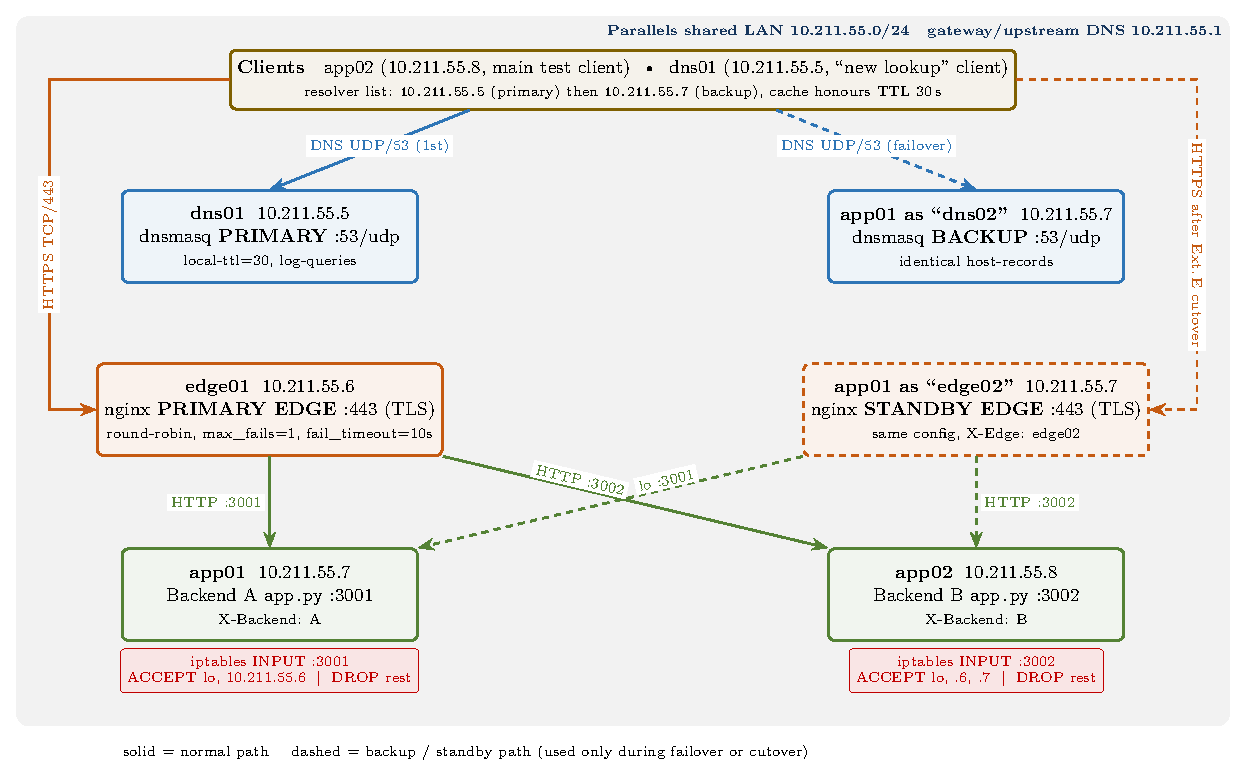
\includegraphics[width=0.86\textwidth]{phase2_topology.pdf}
\caption{Phase~2 topology. Solid arrows are the normal path; dashed arrows are used only during DNS failover or the
edge cutover. Red boxes are the backend firewall allow-lists of Extension~C.}
\label{fig:topo}
\end{figure*}

\begin{table}[!t]
\caption{Machine Roles and IP/Service Inventory}
\label{tab:roles}
\centering\footnotesize
\begin{tabularx}{\columnwidth}{@{}l l Y@{}}
\toprule
VM & IP & Phase~1 role $\rightarrow$ \textbf{added in Phase~2}\\
\midrule
dns01  & .5 & Primary DNS (dnsmasq :53) $\rightarrow$ \textbf{TTL 30\,s, query log; second test client}\\
edge01 & .6 & nginx edge, TLS :443, round-robin $\rightarrow$ \textbf{health checks, retry, X-Edge/X-Upstream}\\
app01  & .7 & Backend A :3001 $\rightarrow$ \textbf{backup DNS ``dns02'' :53, standby edge ``edge02'' :443, firewall on 3001}\\
app02  & .8 & Backend B :3002 $\rightarrow$ \textbf{main test client (resolvers .5, .7), firewall on 3002}\\
\bottomrule
\end{tabularx}
\end{table}

\subsection{DNS Layer}
The Phase~1 dnsmasq file answered with TTL~0, so no client ever cached an answer, which made the TTL experiments of
Extensions B and E impossible. Listing~\ref{lst:dns} shows the Phase~2 primary configuration~\cite{dnsmasq}; dns02 on app01 uses the
same file with \cmd{listen-address=10.211.55.7}. Table~\ref{tab:dnschg} explains each change.

\begin{lstlisting}[caption={Phase~2 dnsmasq configuration on dns01},label={lst:dns}]
listen-address=10.211.55.5
bind-interfaces
no-resolv
server=10.211.55.1
domain-needed
bogus-priv
local=/cn.test/
local-ttl=30
log-queries
host-record=app.cn.test,10.211.55.6
host-record=api.cn.test,10.211.55.6
\end{lstlisting}

\begin{table}[!t]
\caption{dnsmasq Changes from Phase~1}
\label{tab:dnschg}
\centering\footnotesize
\begin{tabularx}{\columnwidth}{@{}>{\raggedright\arraybackslash}p{2.75cm} Y@{}}
\toprule
Directive & Reason\\
\midrule
\cmd{host-record=} & Replaces the wildcard \cmd{address=}; one exact A record, like a zone entry\\
\cmd{local-ttl=30} & Clients may cache answers for 30\,s (Phase~1: 0\,s)\\
\cmd{local=/cn.test/} & Unknown \cmd{*.cn.test} names get NXDOMAIN locally and are never leaked upstream\\
\cmd{no-resolv} & Avoids the loop dns01 $\rightarrow$ 127.0.0.53 $\rightarrow$ systemd-resolved $\rightarrow$ dnsmasq\\
\cmd{domain-needed}, \cmd{bogus-priv} & Standard forwarder hygiene\\
\cmd{log-queries} & Proves which DNS server answered (Extension~A)\\
\bottomrule
\end{tabularx}
\end{table}

The clients (app02 and dns01) now list both resolvers; \cmd{resolvectl status} on app02 reports
\cmd{DNS Servers: 10.211.55.5 10.211.55.7}.

\subsection{Edge Layer}
Listing~\ref{lst:nginx} shows the parts of the edge01 nginx configuration that changed; the TLS server block,
certificate and HTTP-to-HTTPS redirect are unchanged from Phase~1. edge02 uses the same file with
\cmd{X-Edge edge02}.

\begin{lstlisting}[caption={Phase~2 additions to the nginx site on edge01},label={lst:nginx}]
log_format cn_upstream '$remote_addr [$time_local] "$request" $status '
  'upstream=$upstream_addr ustatus=$upstream_status '
  'urt=$upstream_response_time rt=$request_time';
upstream cn_backends {
  server 10.211.55.7:3001 max_fails=1 fail_timeout=10s;
  server 10.211.55.8:3002 max_fails=1 fail_timeout=10s;
}
# inside the :443 server block
access_log /var/log/nginx/cn_access.log cn_upstream;
error_log  /var/log/nginx/cn_error.log warn;
add_header X-Edge edge01 always;
add_header X-Upstream $upstream_addr always;
location / {
  proxy_pass http://cn_backends;
  proxy_connect_timeout 2s;
  proxy_read_timeout 5s;
  proxy_next_upstream error timeout http_502 http_503 http_504;
  proxy_next_upstream_tries 2;
  proxy_next_upstream_timeout 5s;
  ...
}
\end{lstlisting}

\cmd{max\_fails=1 fail\_timeout=10s} is a passive health check: after one failed attempt the server is skipped for
10\,s~\cite{nginxup}. A 2\,s connect timeout replaces the 60\,s default, and \cmd{proxy\_next\_upstream} retries a failed
request once on the other backend, which is safe because \cmd{GET} is idempotent~\cite{rfc9110}. The \cmd{X-Upstream}
and \cmd{X-Edge} headers expose which backends were tried and which edge answered.

\subsection{Backend Firewalls}
Ubuntu's equivalent of the macOS \cmd{pf} firewall is iptables~\cite{iptables}. Three rules are inserted at the top of
\cmd{INPUT} on each backend, only for the backend port (Listing~\ref{lst:fw}); SSH and DNS are untouched. app02 uses port 3002, and a fourth rule there admits edge02
(\cmd{-s 10.211.55.7}) for the cutover. The original rule set was saved to
\cmd{/root/phase1-backup/iptables-before-ext-c.rules} before any change.

\begin{lstlisting}[caption={Service-isolation rules on app01},label={lst:fw}]
iptables -I INPUT 1 -i lo -p tcp --dport 3001 -j ACCEPT
iptables -I INPUT 2 -s 10.211.55.6 -p tcp --dport 3001 -j ACCEPT
iptables -I INPUT 3 -p tcp --dport 3001 -j DROP
\end{lstlisting}

\subsection{Request Flow}
Fig.~\ref{fig:flow} traces one request through each protocol layer (DNS~\cite{rfc1035}, TCP~\cite{rfc9293}, TLS~\cite{rfc8446} and HTTP~\cite{rfc9110}) together with the Phase~2 failure paths.

\begin{figure*}[!t]
\centering
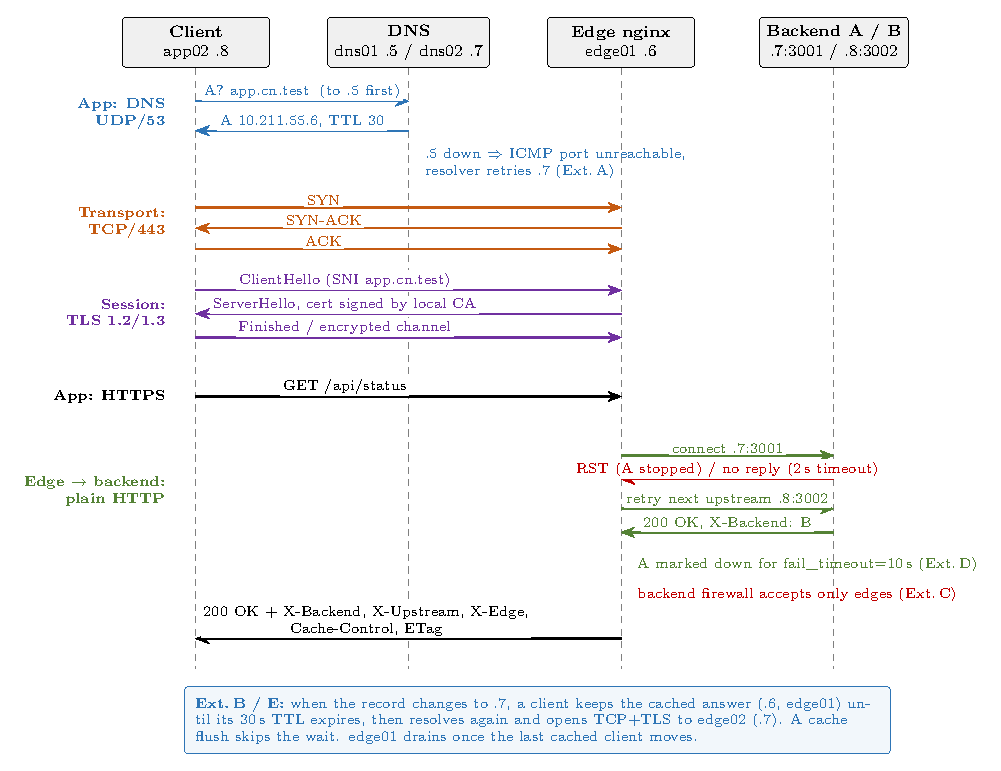
\includegraphics[width=0.72\textwidth]{phase2_request_flow.pdf}
\caption{Phase~2 request flow per protocol layer: DNS with failover, TCP and TLS to the edge, HTTP behind the edge
with retry on the next upstream.}
\label{fig:flow}
\end{figure*}

% =====================================================================
\section{Resilience Tests and Results}\label{sec:tests}
Unless stated otherwise, tests were run from app02. Each subsection gives the goal, procedure, expected and observed
results, and the evidence. The evidence files are in \cmd{phase-2/evidence/}.

% ---------------------------------------------------------------------
\subsection{Extension A: Backup DNS Resolver}
\emph{Goal.} A second resolver with the same records keeps names resolving when the primary DNS service stops, and the
difference between a DNS failure and an application failure is shown.

\emph{Procedure.} dns02 was tested directly first: \cmd{dig @10.211.55.7 app.cn.test} returned
\cmd{30 IN A 10.211.55.6} from \cmd{SERVER: 10.211.55.7\#53} (Fig.~\ref{fig:a-direct}). With \cmd{journalctl -f} running
on both DNS servers and \cmd{tcpdump} on app02, a baseline lookup was made, dnsmasq was stopped on dns01 only, the
client cache was flushed and the lookup was repeated.

\emph{Expected.} The primary refuses the query, the client retries the backup, the name still resolves to
\cmd{10.211.55.6}, and HTTPS keeps working.

\emph{Observed} (Fig.~\ref{fig:a-failover}). The baseline query at 00:59:58 appears in the dns01 log. After dnsmasq
stopped at 01:00:11, \cmd{dig @10.211.55.5} reported \cmd{connection refused} and \cmd{no servers could be reached}.
After a flush, \cmd{dig app.cn.test} still returned \cmd{10.211.55.6} at 01:00:52, the query appeared only in the
app01 (dns02) log, \cmd{resolvectl} reported \cmd{Current DNS Server: 10.211.55.7}, and four HTTPS requests returned
\cmd{200} alternating between Backend~A and~B. In \cmd{phase2\_dns\_failover.pcapng} the query to \cmd{.5} (frame~9)
is answered by \emph{ICMP Destination unreachable (Port unreachable)} (frames 10--16): the host is up but nothing
listens on UDP/53. The next query goes to \cmd{.7} and is answered with \cmd{10.211.55.6} (frames 23--24).

\begin{figure}[!t]
\centering
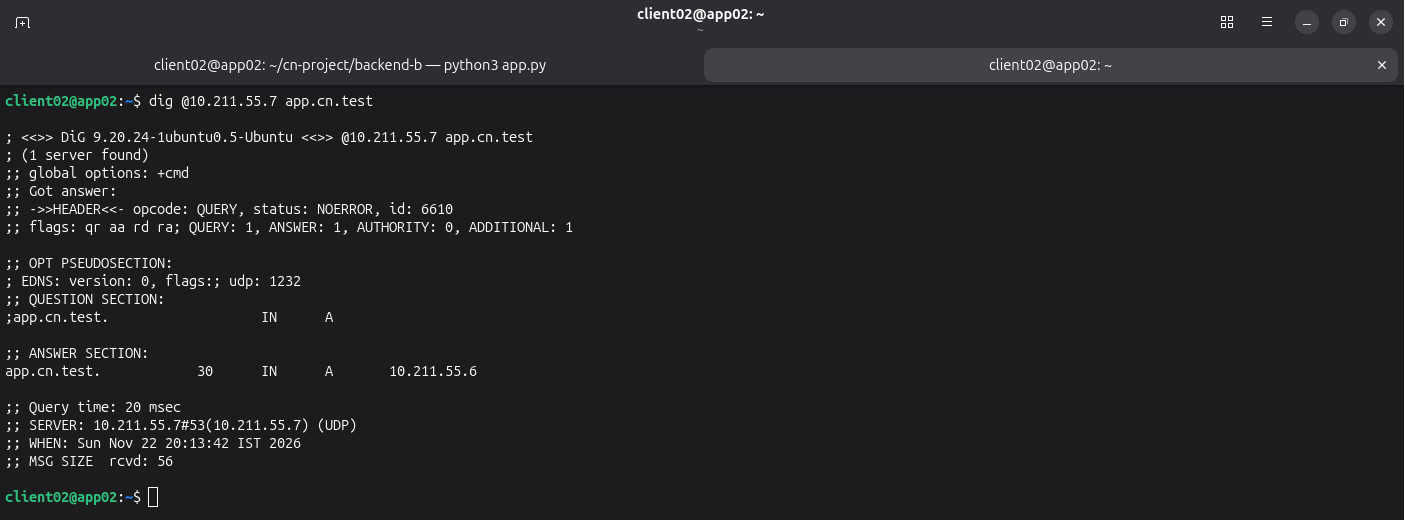
\includegraphics[width=\columnwidth]{p2_fig03_dns02_direct.png}
\caption{Backup resolver dns02 (10.211.55.7) answers \cmd{app.cn.test} with the same record and TTL~30.}
\label{fig:a-direct}
\end{figure}

\begin{figure*}[!t]
\centering
\subfloat[dns01 log: last query at 00:59:59, then dnsmasq stopped]{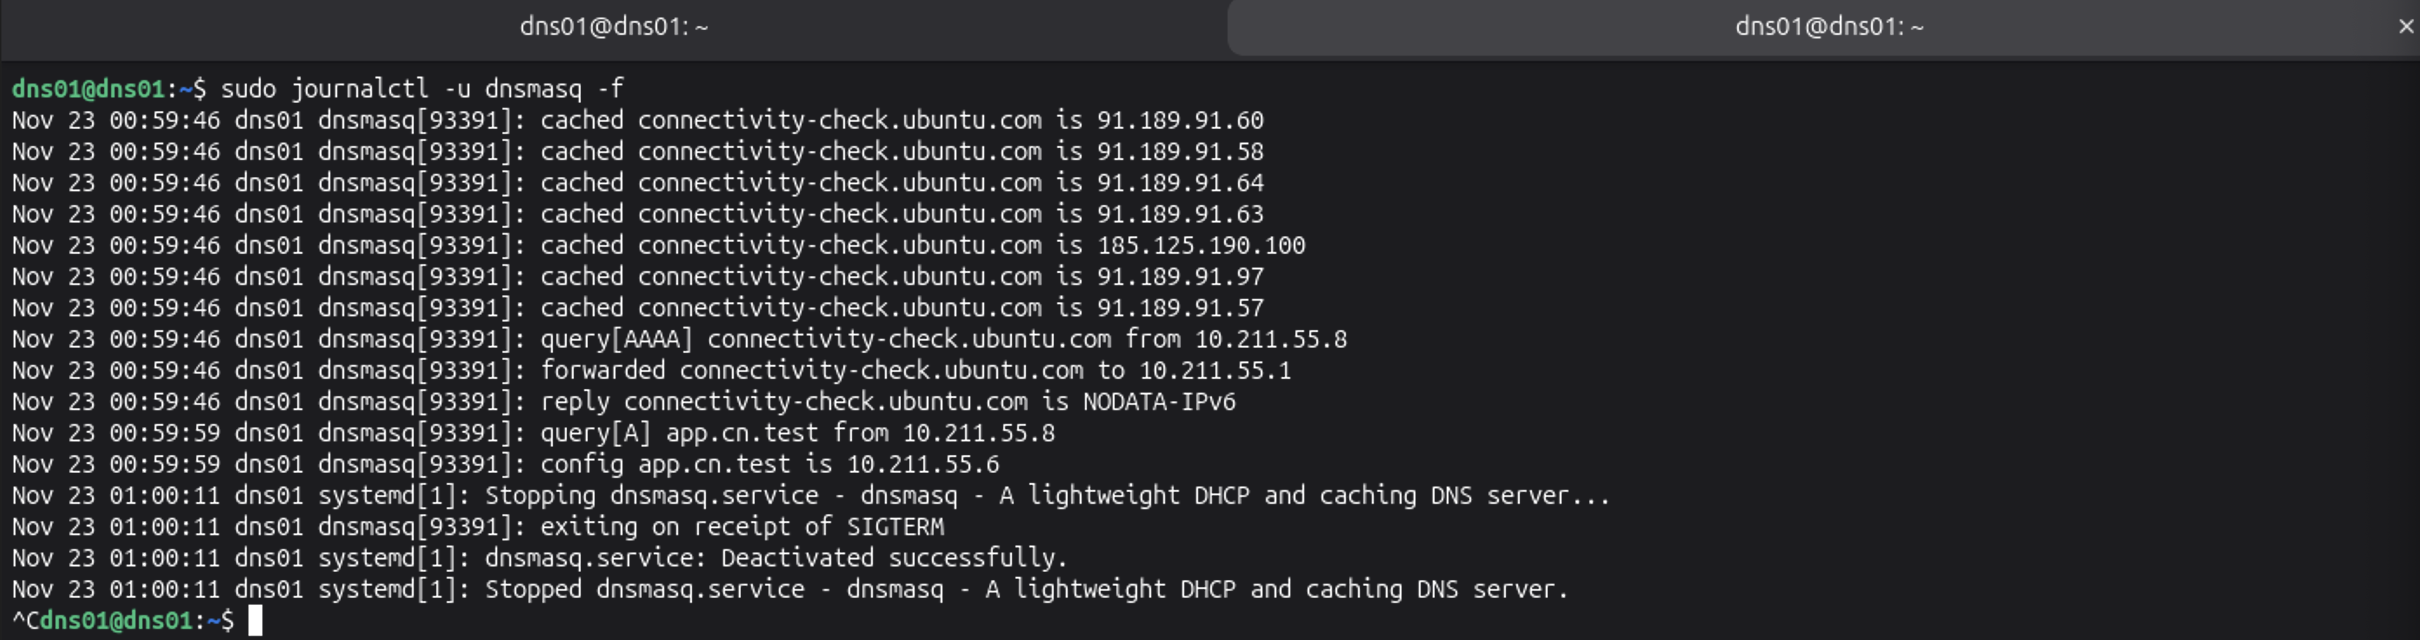
\includegraphics[width=0.49\textwidth]{p2_fig05a_dns01_log.png}}\hfill
\subfloat[app01/dns02 log: later queries are answered by the backup]{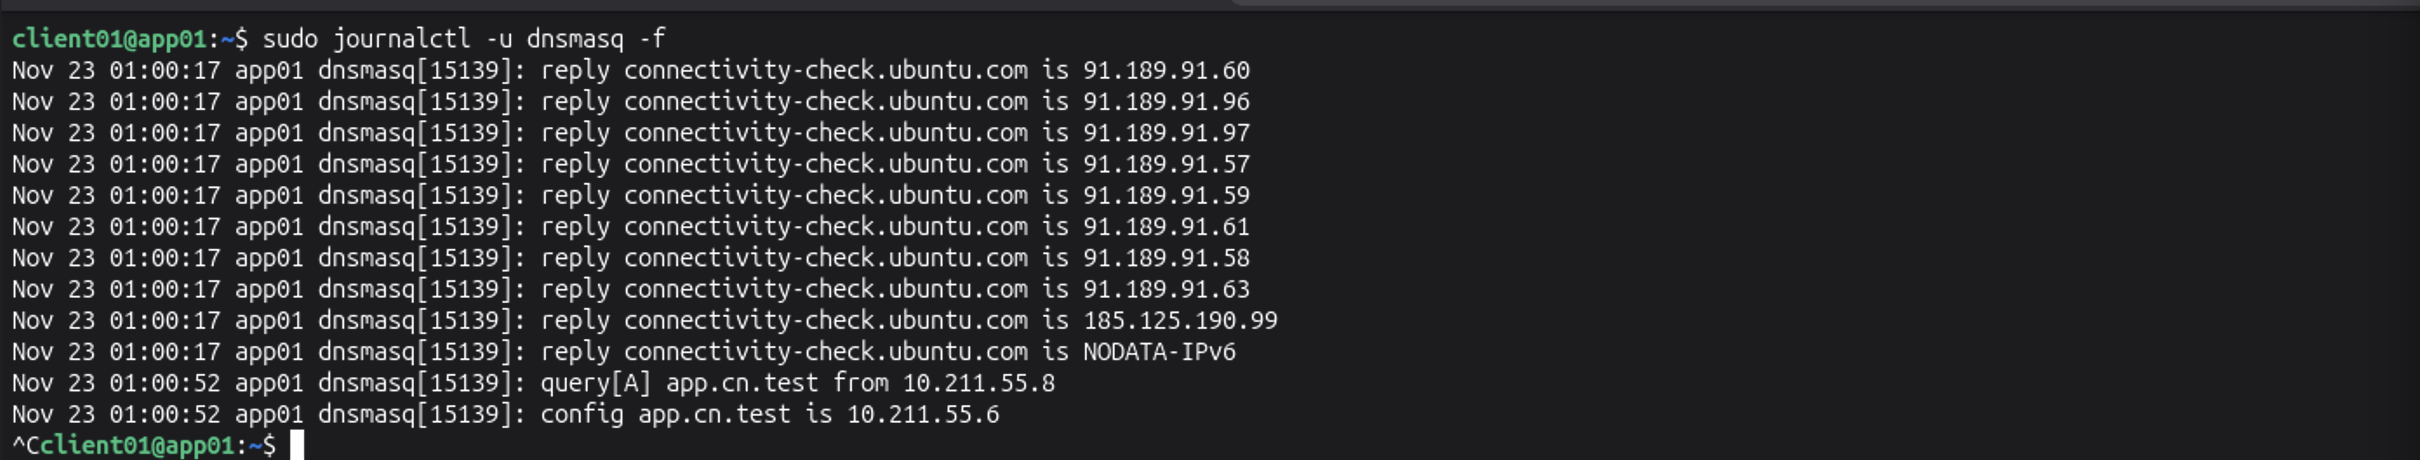
\includegraphics[width=0.49\textwidth]{p2_fig05b_app01_log.png}}\\
\subfloat[app02 client: primary refused, lookup still succeeds via 10.211.55.7, HTTPS still served by A and B]{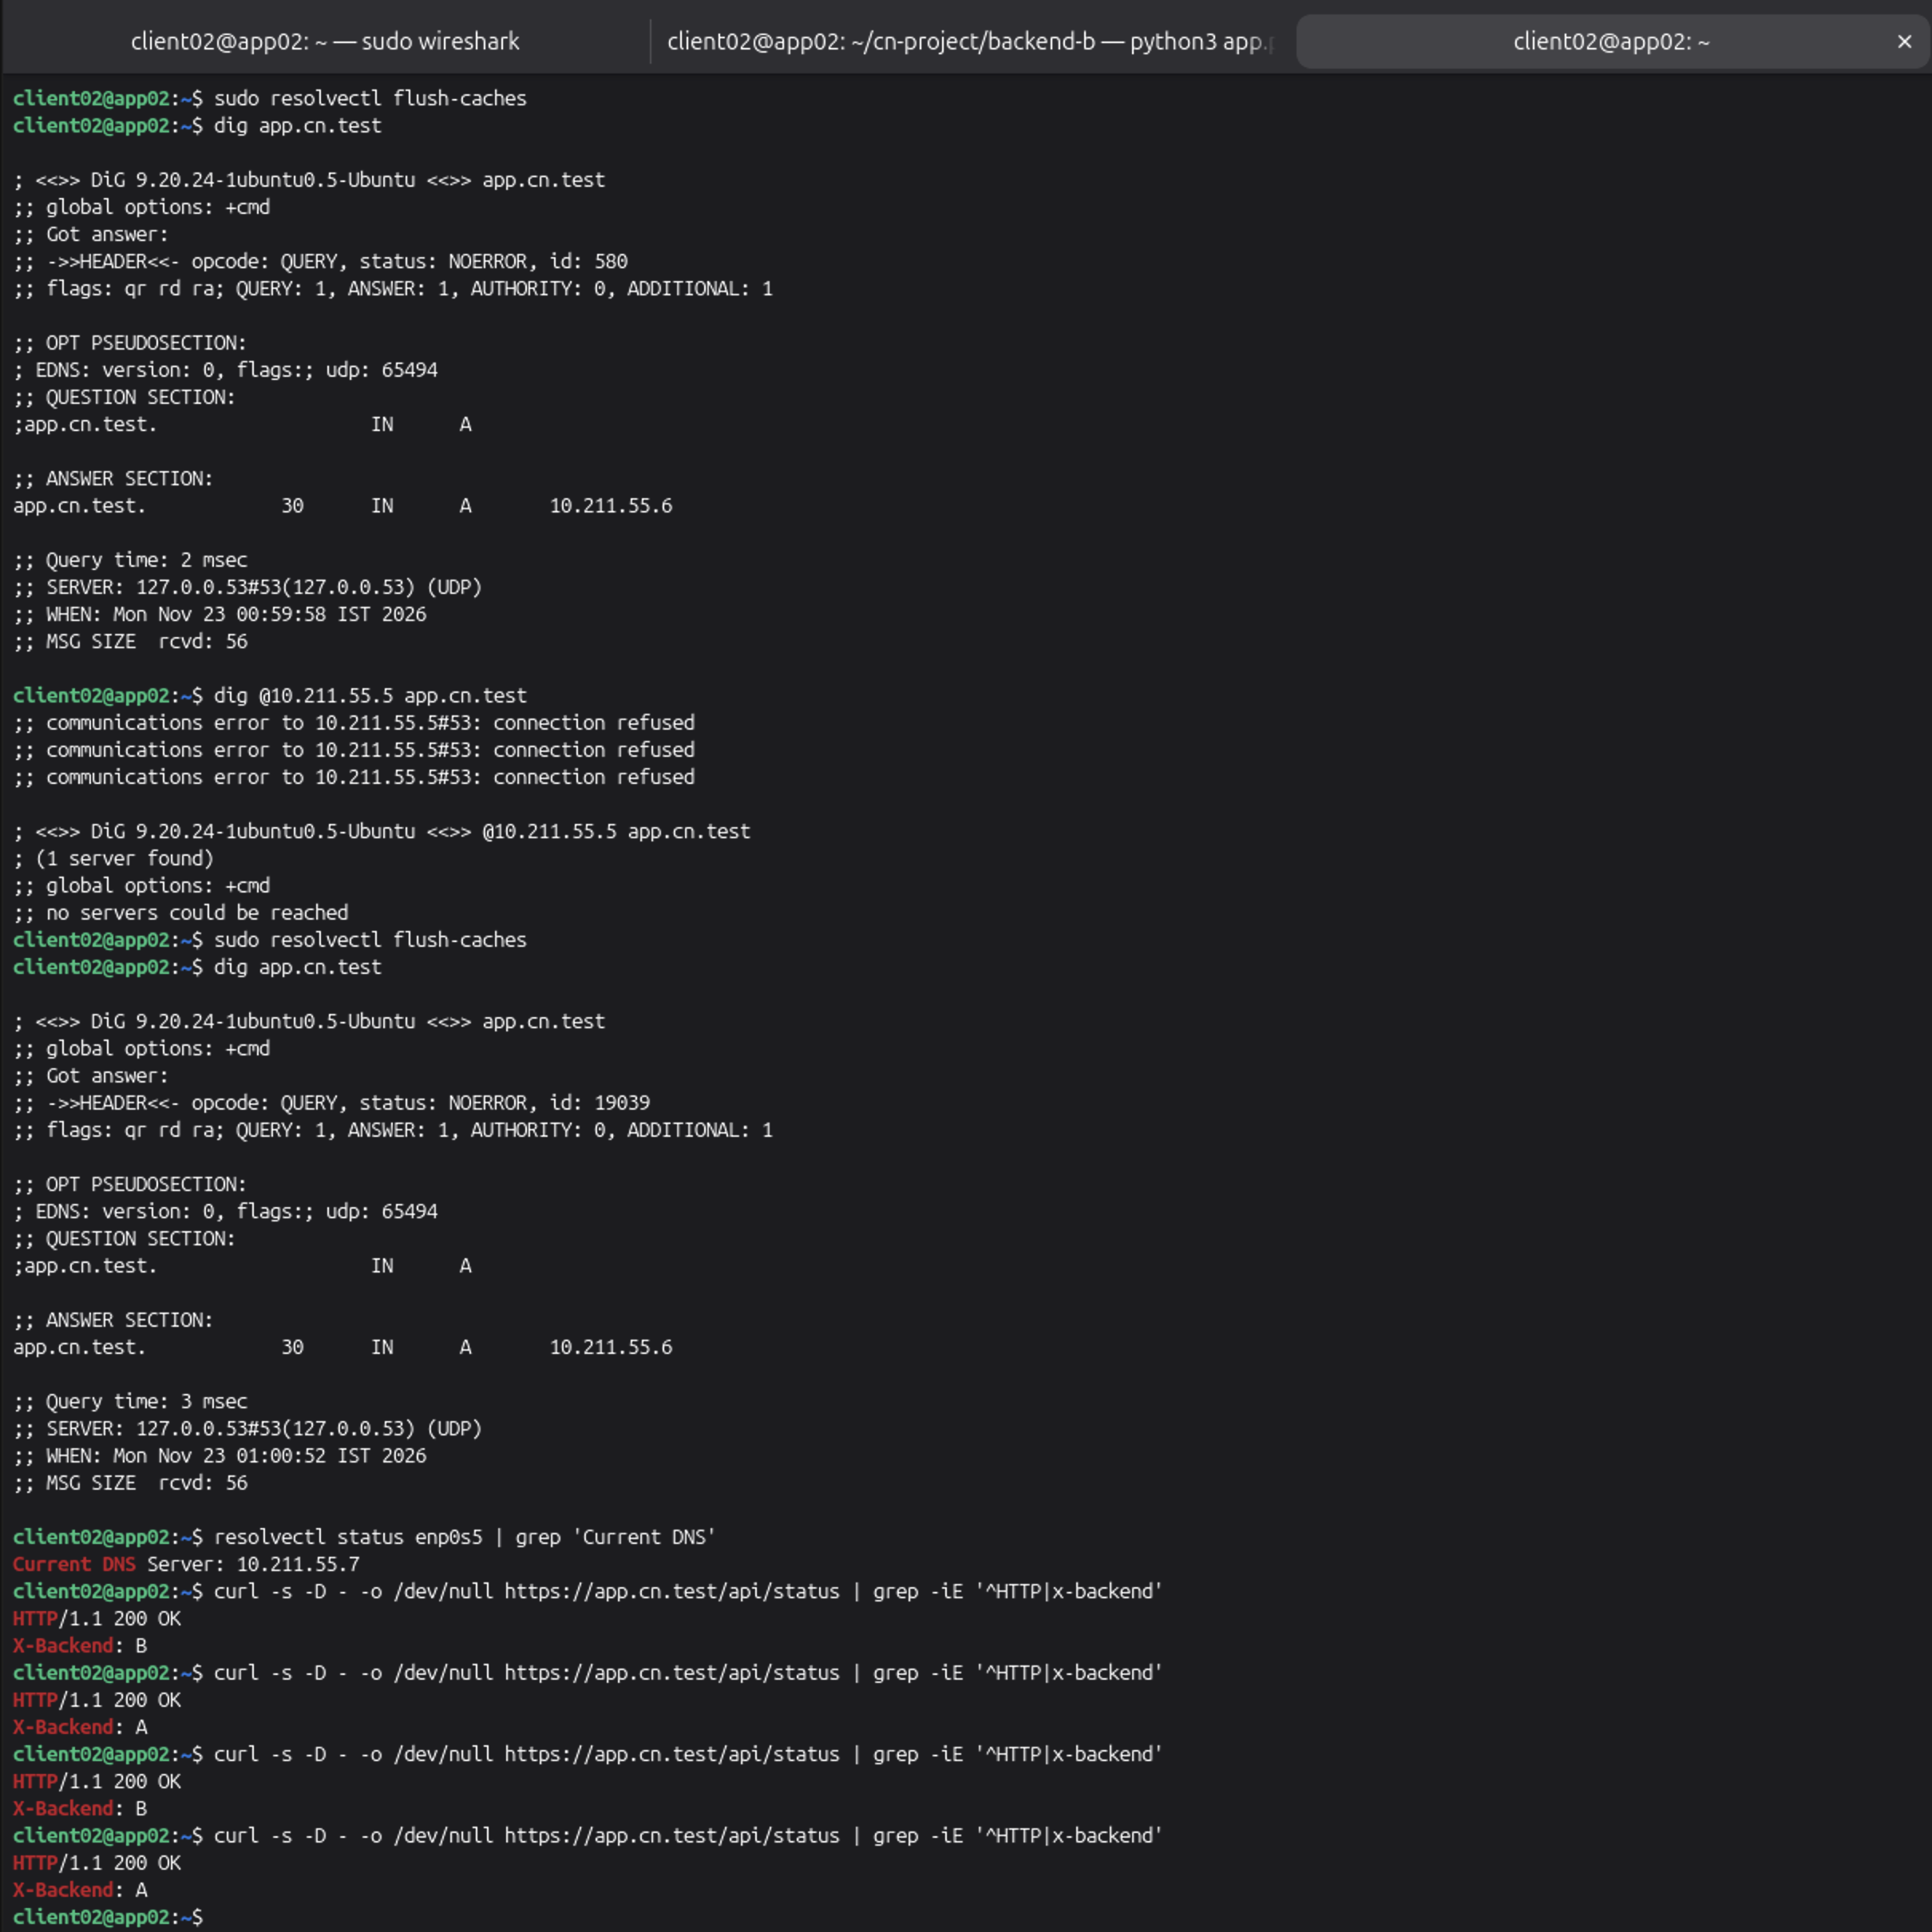
\includegraphics[width=0.55\textwidth]{p2_fig05c_app02_client.png}}
\caption{Extension~A failover with the primary DNS service stopped (\cmd{p2\_fig05\_dns\_failover.png}).}
\label{fig:a-failover}
\end{figure*}

\emph{DNS failure versus application failure.} With dnsmasq stopped on \emph{both} servers, curl failed with
\cmd{(6) Could not resolve host} and HTTP code \cmd{000}, while \cmd{ping 10.211.55.6} succeeded (Fig.~\ref{fig:a-dnsfail}):
the service was healthy but could not be named. With DNS working and both backends stopped, \cmd{dig} returned
\cmd{10.211.55.6} and nginx answered \cmd{502 Bad Gateway} (Fig.~\ref{fig:a-appfail}): DNS, TCP and TLS worked and the
failure was behind the edge. Table~\ref{tab:dnsvsapp} summarises the contrast.

\begin{figure}[!t]
\centering
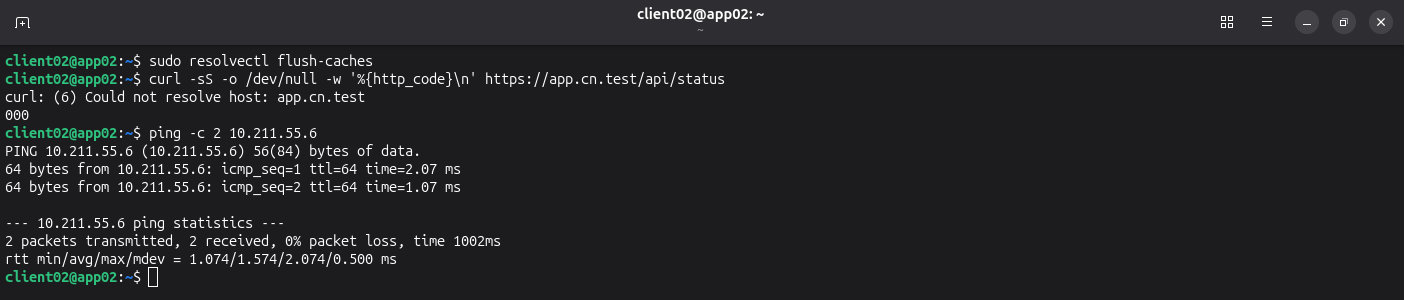
\includegraphics[width=\columnwidth]{p2_fig06_dns_failure.png}
\caption{DNS service failure: name resolution fails although the edge answers ping.}
\label{fig:a-dnsfail}
\end{figure}

\begin{figure}[!t]
\centering
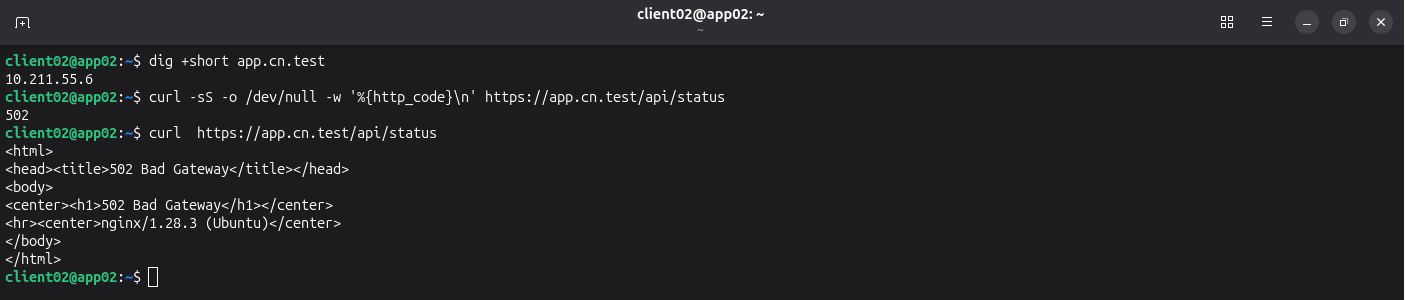
\includegraphics[width=\columnwidth]{p2_fig07_app_failure.png}
\caption{Application failure: DNS resolves, nginx returns 502 because no backend is up.}
\label{fig:a-appfail}
\end{figure}

\begin{table}[!t]
\caption{DNS Failure Versus Application Failure}
\label{tab:dnsvsapp}
\centering\footnotesize
\begin{tabular}{@{}lll@{}}
\toprule
Check & DNS failure & Application failure\\
\midrule
\cmd{dig app.cn.test} & fails & 10.211.55.6\\
TCP/TLS to edge & never attempted & succeed\\
HTTP result & none (\cmd{000}) & \cmd{502} from nginx\\
Meaning & name $\not\rightarrow$ address & failure is behind the edge\\
\bottomrule
\end{tabular}
\end{table}

% ---------------------------------------------------------------------
\subsection{Extension B: DNS TTL and Controlled Record Change}
\emph{Goal.} Use a short visible TTL, change a record and show that a client keeps the cached answer until the TTL
expires, and that a manual flush applies the change immediately.

\emph{TTL before and after.} In Phase~1 the answer carried TTL~0 (Fig.~\ref{fig:b-ttl}a); after the change it carries
TTL~30 (Fig.~\ref{fig:b-ttl}b). Two lookups through the local stub resolver ten seconds apart returned TTL~30 and then
TTL~20 (Fig.~\ref{fig:b-ttl}c). The countdown proves the second answer came from the client cache, because the
server always sends~30.

\begin{figure}[!t]
\centering
\subfloat[Phase~1: TTL 0]{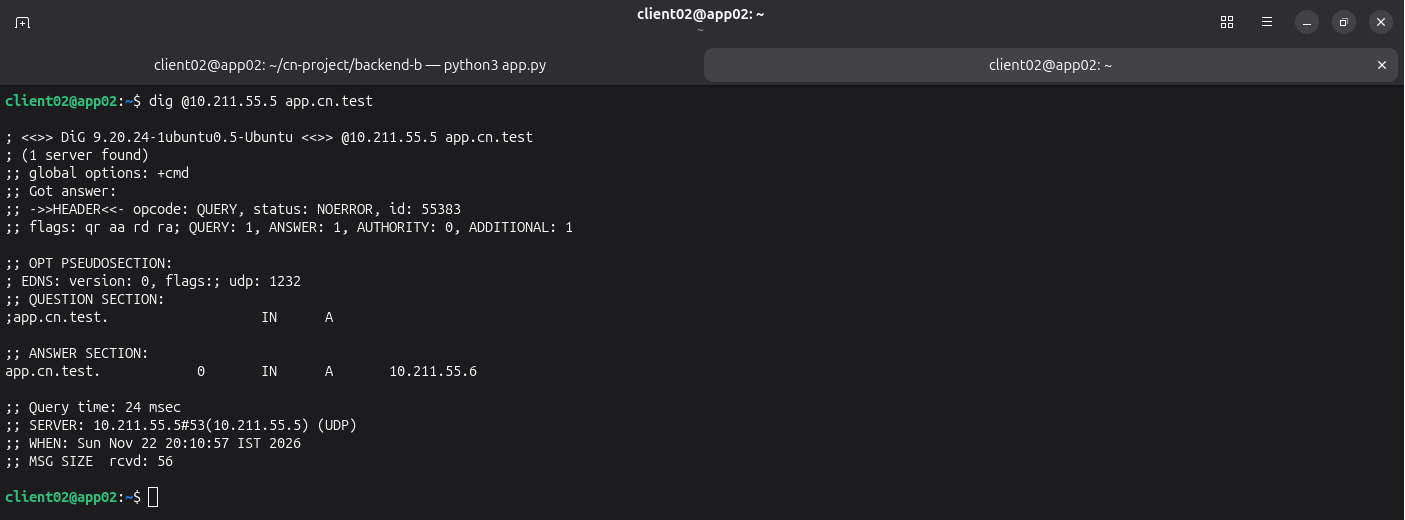
\includegraphics[width=\columnwidth]{p2_fig01_ttl0_before.png}}\\
\subfloat[Phase~2: TTL 30]{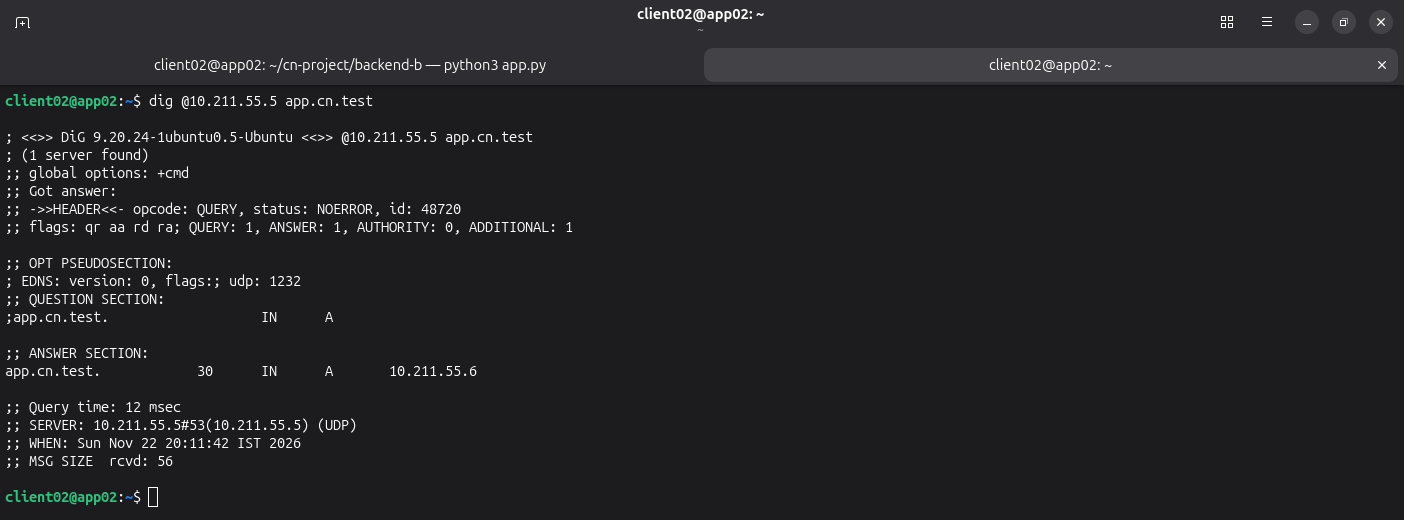
\includegraphics[width=\columnwidth]{p2_fig02_ttl30_after.png}}\\
\subfloat[Cached answer counting down 30 $\rightarrow$ 20]{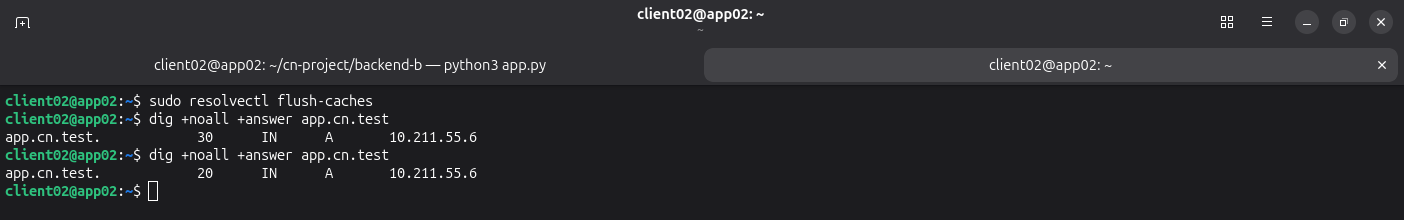
\includegraphics[width=\columnwidth]{p2_fig08_ttl_countdown.png}}
\caption{Record TTL before and after the change, and client-side caching.}
\label{fig:b-ttl}
\end{figure}

\emph{Record change.} A loop on app02 printed, every 2\,s, the cached answer with its remaining TTL and the server's
live answer. The record was then changed from \cmd{.6} to \cmd{.7} on both DNS servers. From 01:26:16 the server
answered \cmd{10.211.55.7}, but the client kept returning the cached \cmd{10.211.55.6} with TTL 11, 9, 7, 5, 3 and 1\,s.
At 01:26:28, once the TTL had expired, the client fetched the new answer \cmd{30s -> 10.211.55.7} (Fig.~\ref{fig:b-change}).
Clients therefore lag a change by at most one TTL; here the lag was about 12\,s because the change landed late in the
cache period.

\begin{figure}[!t]
\centering
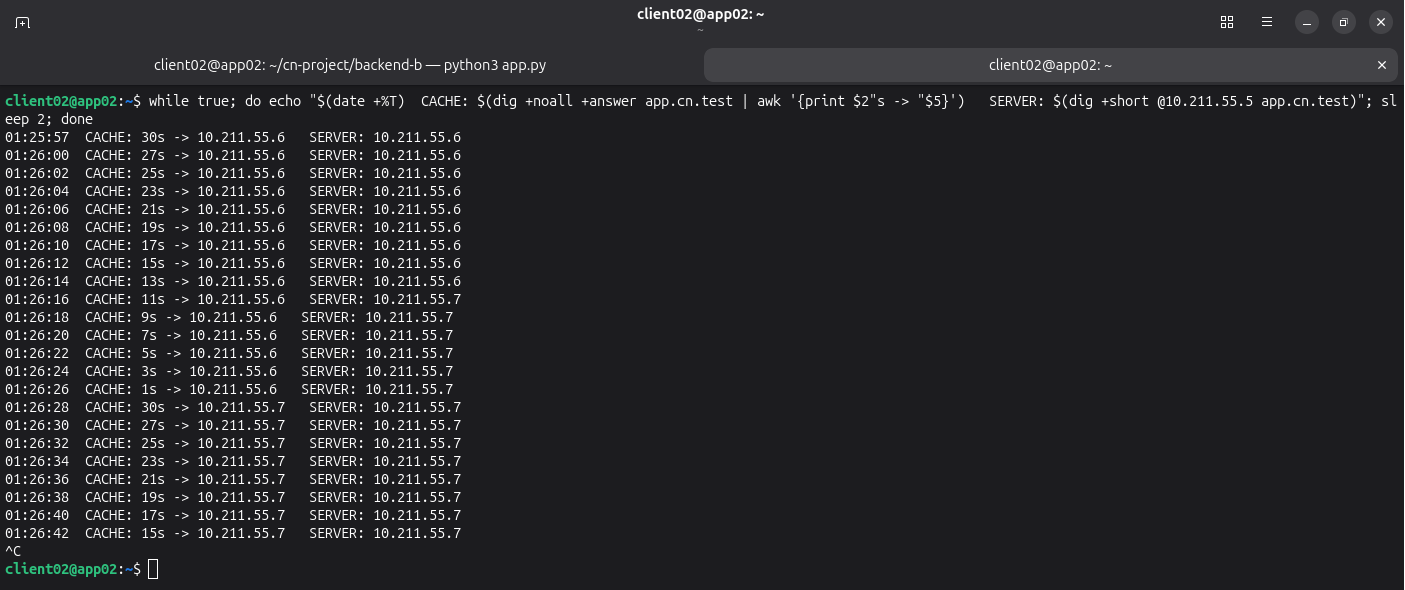
\includegraphics[width=\columnwidth]{p2_fig09_ttl_record_change.png}
\caption{Record change: the server switches to .7 at 01:26:16, the cached client follows only at TTL expiry (01:26:28).}
\label{fig:b-change}
\end{figure}

\emph{Manual flush.} With \cmd{10.211.55.7} cached and the record already restored to \cmd{.6}, running
\cmd{sudo resolvectl flush-caches} made the very next lookup return \cmd{30 IN A 10.211.55.6} with no waiting
(Fig.~\ref{fig:b-flush}). \cmd{resolvectl statistics} reported 61 cache hits and 334 misses for the session.

\begin{figure}[!t]
\centering
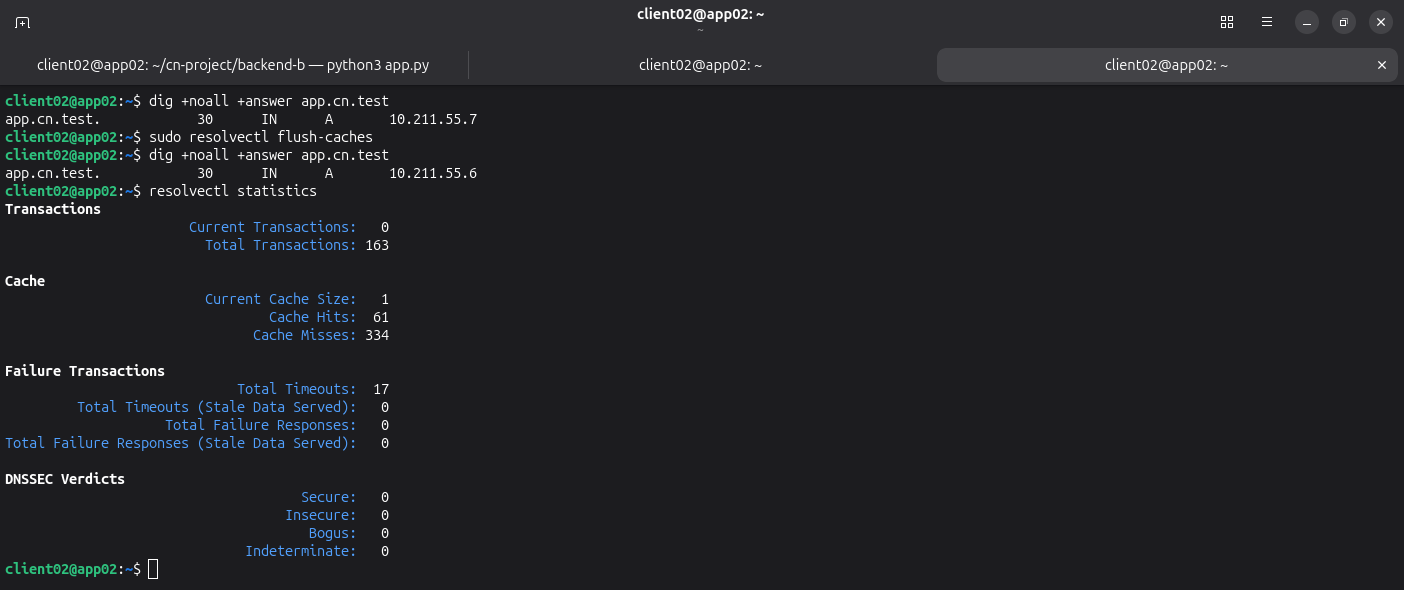
\includegraphics[width=\columnwidth]{p2_fig10_dns_flush.png}
\caption{Manual cache flush: the new answer is returned immediately.}
\label{fig:b-flush}
\end{figure}

% ---------------------------------------------------------------------
\subsection{Extension C: Service Isolation (Backend Firewall)}
\emph{Goal.} Only the edge may reach ports 3001 and 3002; clients must be blocked; the original rules must be restored.

\emph{Before.} dns01 connected directly to both backends (\cmd{nc -vz}: \cmd{succeeded}, Fig.~\ref{fig:c-before}).
The saved rule sets contained no INPUT rules on either backend.

\emph{Rules.} Listing~\ref{lst:fw} was applied on app01 and its equivalent on app02 (Fig.~\ref{fig:c-rules}).
Rules are evaluated top to bottom and the first match wins, so the specific ACCEPT rules precede the DROP.

\emph{After} (Fig.~\ref{fig:c-after}). From dns01 both ports \cmd{timed out}, and from app02 port 3001 also
\cmd{timed out}. edge01 still \cmd{succeeded} to both backends, and HTTPS through the edge kept alternating between
A and~B. DROP produces a timeout rather than a refusal because no RST is sent; the client only retransmits its SYN.

\begin{figure}[!t]
\centering
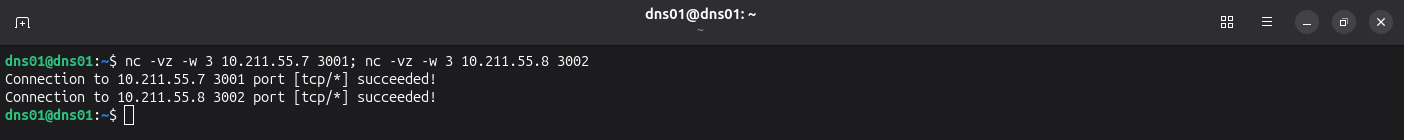
\includegraphics[width=\columnwidth]{p2_fig15_before_isolation.png}
\caption{Before isolation: a client reaches both backend ports directly.}
\label{fig:c-before}
\end{figure}

\begin{figure}[!t]
\centering
\subfloat[app01, port 3001]{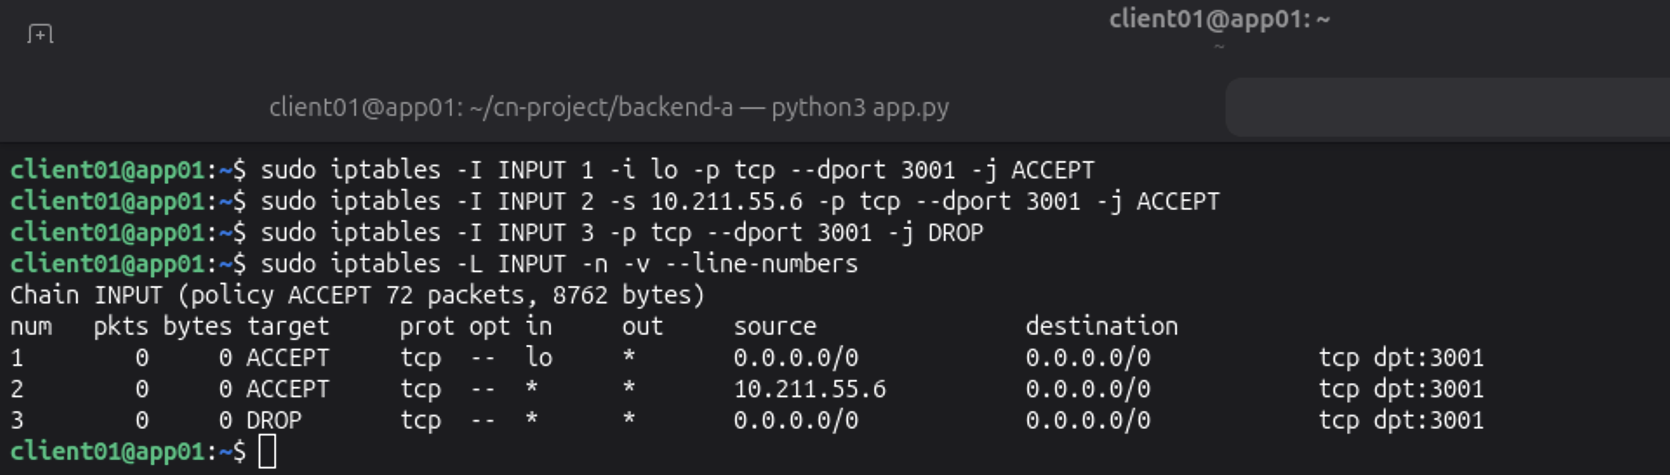
\includegraphics[width=\columnwidth]{p2_fig16a_app01.png}}\\
\subfloat[app02, port 3002]{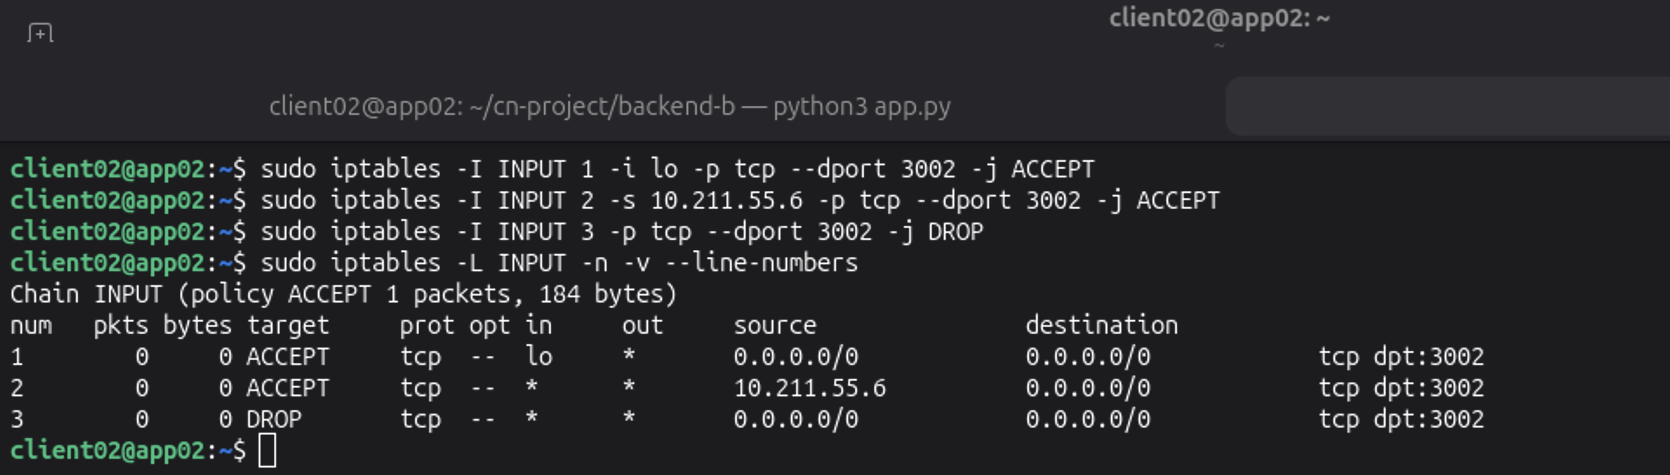
\includegraphics[width=\columnwidth]{p2_fig16b_app02.png}}
\caption{Firewall rules: loopback and edge01 accepted, everything else dropped.}
\label{fig:c-rules}
\end{figure}

\begin{figure}[!t]
\centering
\subfloat[Client dns01: both ports time out]{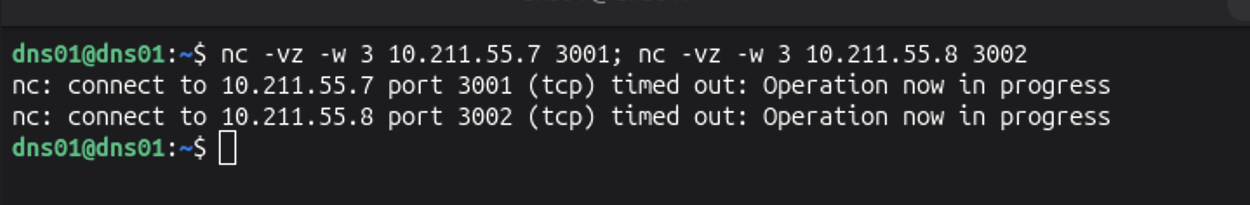
\includegraphics[width=\columnwidth]{p2_fig17a_dns01.png}}\\
\subfloat[Client app02: port 3001 times out]{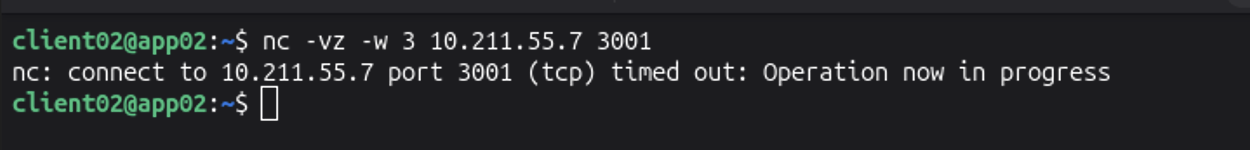
\includegraphics[width=\columnwidth]{p2_fig17b_app02.png}}\\
\subfloat[Edge edge01: both ports still reachable]{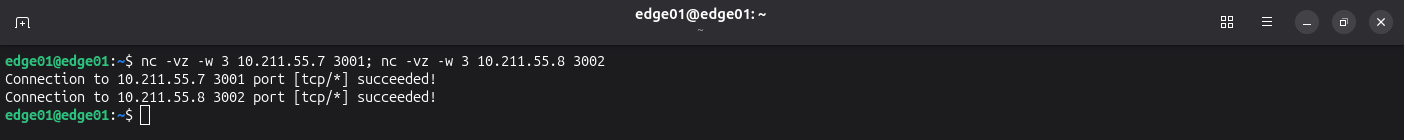
\includegraphics[width=\columnwidth]{p2_fig18_edge_allowed.png}}
\caption{Isolation verified from the client side and the edge side.}
\label{fig:c-after}
\end{figure}

\emph{Rollback.} After Extension~E, exactly the added rules were deleted with \cmd{iptables -D} (three on app01, four on
app02). \cmd{iptables-save} then showed no INPUT rules, identical to the saved copy, and dns01 reached both ports again
(Fig.~\ref{fig:c-rollback}). The saved, applied and final rule sets are in \cmd{vm\_logs/app0\{1,2\}/}.

\begin{figure}[!t]
\centering
\subfloat[app01: rules removed, no difference from the saved copy]{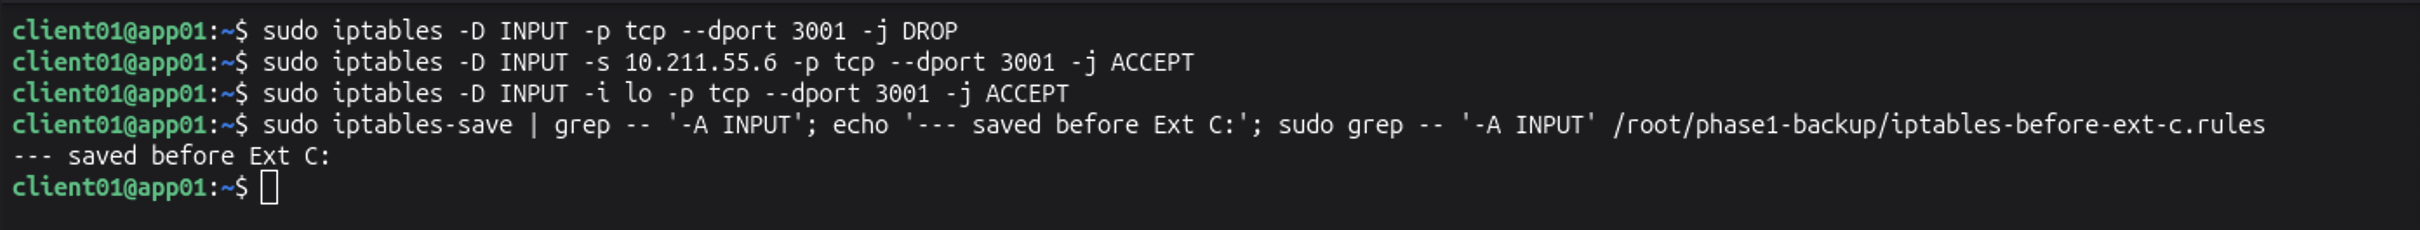
\includegraphics[width=\columnwidth]{p2_fig23a_app01.png}}\\
\subfloat[app02: four rules removed]{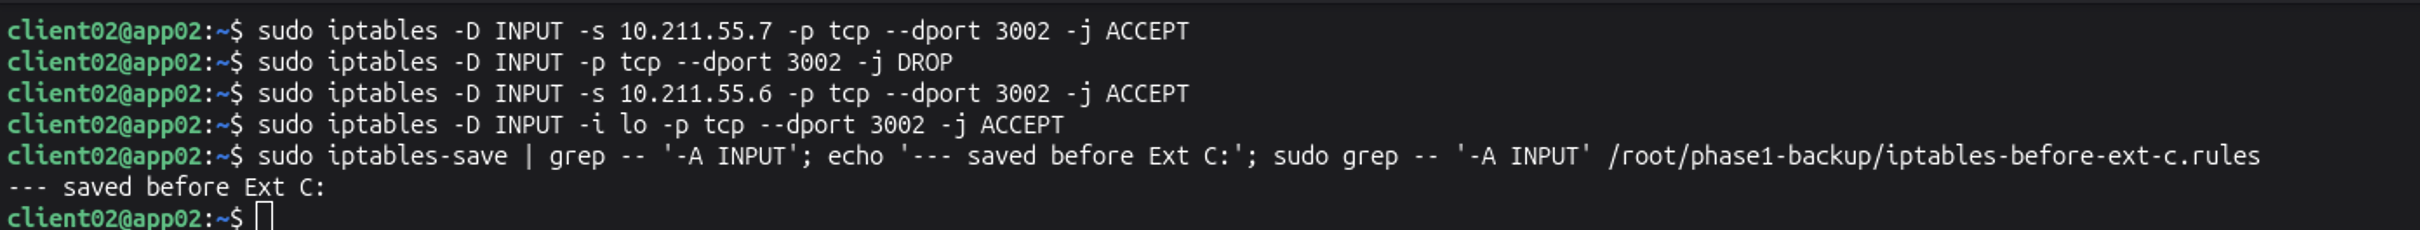
\includegraphics[width=\columnwidth]{p2_fig23b_app02.png}}\\
\subfloat[dns01: direct access restored]{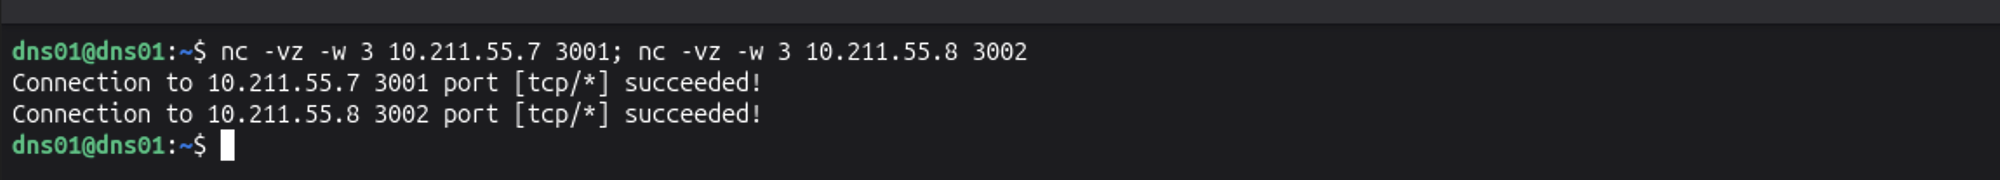
\includegraphics[width=0.85\columnwidth]{p2_fig23c_dns01.png}}
\caption{Firewall rollback to the original configuration.}
\label{fig:c-rollback}
\end{figure}

% ---------------------------------------------------------------------
\subsection{Extension D: High-Availability Failover}
\emph{Goal.} nginx detects an unavailable backend and routes only to the healthy one, then resumes balancing when
it returns.

\emph{Baseline.} Six requests alternated A, B, A, B, A, B with \cmd{X-Upstream} naming one backend each (Fig.~\ref{fig:d-base}).

\emph{Backend A stopped.} All six requests returned \cmd{200} from Backend~B (Fig.~\ref{fig:d-down}). One request shows
\cmd{X-Upstream: 10.211.55.7:3001, 10.211.55.8:3002}: nginx tried A, received a TCP RST, and retried on B within the
same client request. The edge error log records \cmd{connect() failed (111: Connection refused)} followed by
\cmd{upstream server temporarily disabled} (Fig.~\ref{fig:d-log}); the access log shows
\cmd{ustatus=502, 200} for that request and \cmd{upstream=10.211.55.8:3002} only for the following ones. The client
never saw an error.

\emph{Recovery.} After Backend~A restarted and the 10\,s \cmd{fail\_timeout} elapsed, requests alternated between A
and B again (Fig.~\ref{fig:d-rec}).

\begin{figure}[!t]
\centering
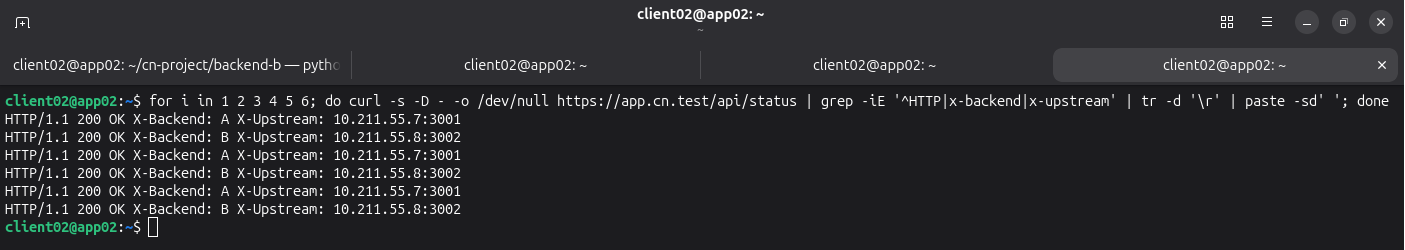
\includegraphics[width=\columnwidth]{p2_fig11_ha_baseline.png}
\caption{Baseline: round-robin across both backends.}
\label{fig:d-base}
\end{figure}

\begin{figure}[!t]
\centering
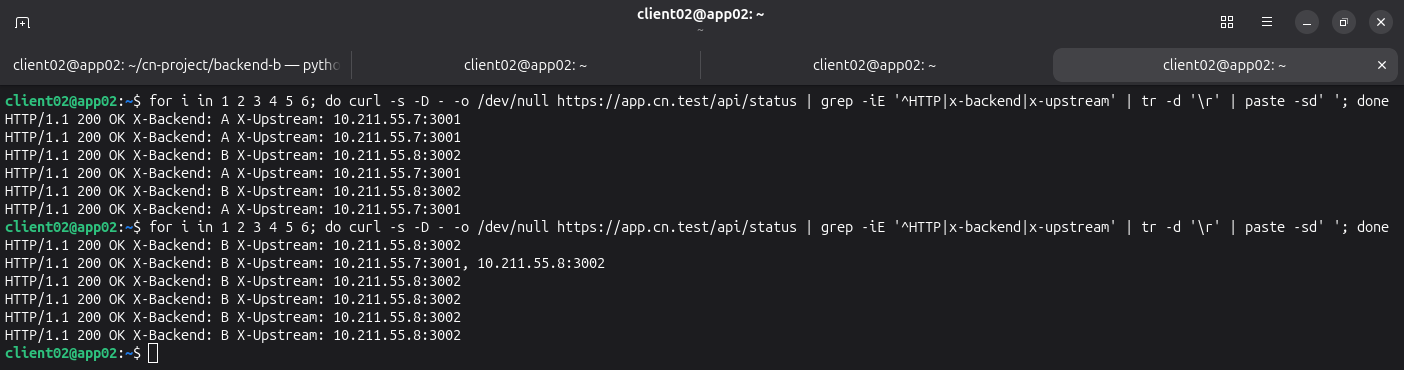
\includegraphics[width=\columnwidth]{p2_fig12_ha_backend_a_down.png}
\caption{Backend~A stopped: every request still succeeds through Backend~B.}
\label{fig:d-down}
\end{figure}

\begin{figure}[!t]
\centering
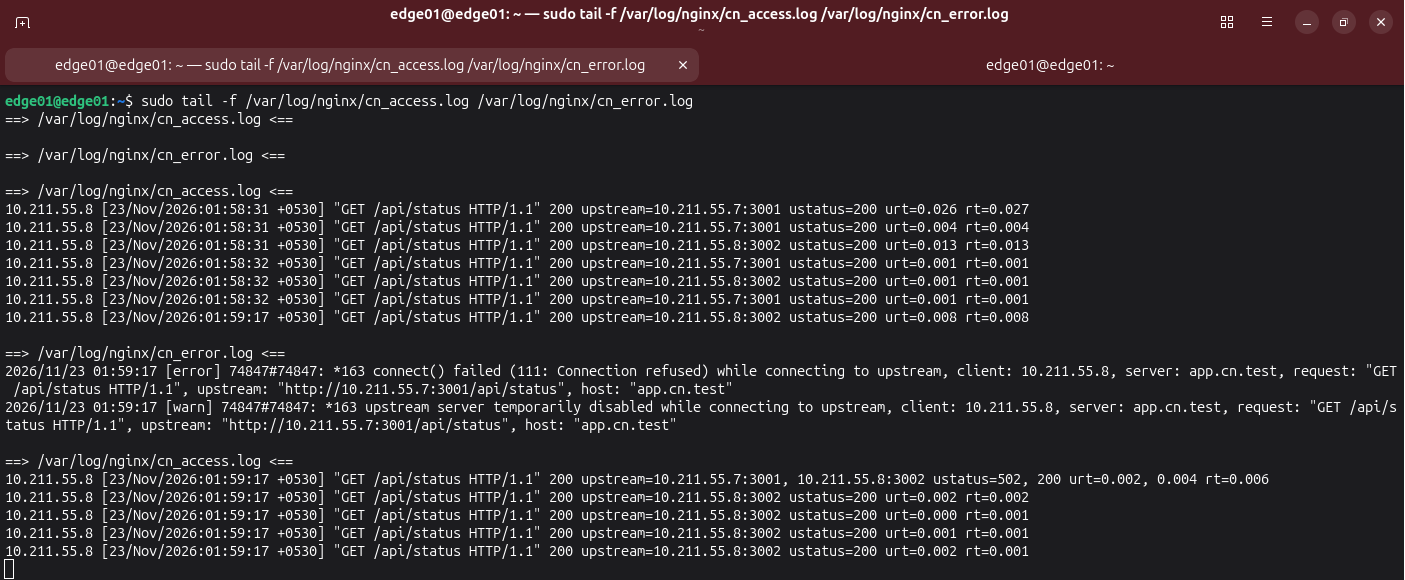
\includegraphics[width=\columnwidth]{p2_fig13_nginx_error_log.png}
\caption{edge01 logs: connection refused by A, A disabled, retry served by B.}
\label{fig:d-log}
\end{figure}

\begin{figure}[!t]
\centering
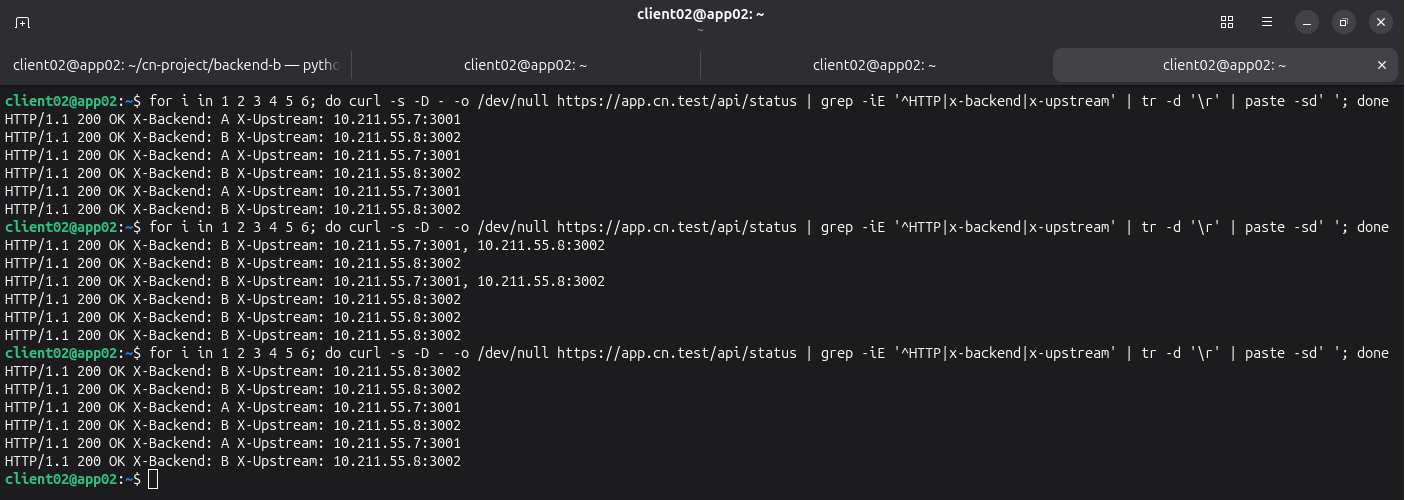
\includegraphics[width=\columnwidth]{p2_fig14_ha_recovery.png}
\caption{Before, during and after the outage: balancing resumes once A is back.}
\label{fig:d-rec}
\end{figure}

\emph{Remaining single point of failure.} DNS (Extension~A) and the backends (Extension~D) are now redundant, but the
edge is not. If edge01 fails, \cmd{app.cn.test} still resolves to \cmd{10.211.55.6} and nothing answers on port~443.
It could be removed by (i) two edges sharing a floating virtual IP using VRRP (keepalived), which fails over in
1--3\,s without any DNS change; (ii) two edges behind DNS failover records, limited by the TTL as Extension~E shows; or
(iii) a managed, multi-zone load balancer.

% ---------------------------------------------------------------------
\subsection{Extension E: Controlled Edge Migration (DNS Cutover)}
\emph{Goal.} Bring up a standby edge with the same configuration, point \cmd{app.cn.test} at it, and show that cached
clients briefly keep using the old edge while new lookups go to the standby.

\emph{Standby edge.} nginx was installed on app01 with the edge01 configuration (only \cmd{X-Edge edge02} differs) and
the same certificate and key. A firewall rule on app02 admitted \cmd{10.211.55.7} to port 3002; without it the
standby edge could only use Backend~A. This is a practical lesson: \emph{an allow-list must include every edge, or a
migration breaks silently}. Before any DNS change, \cmd{curl --resolve app.cn.test:443:10.211.55.7} returned
\cmd{200} with \cmd{X-Edge: edge02} from both backends, with valid TLS (Fig.~\ref{fig:e-direct}).

\begin{figure}[!t]
\centering
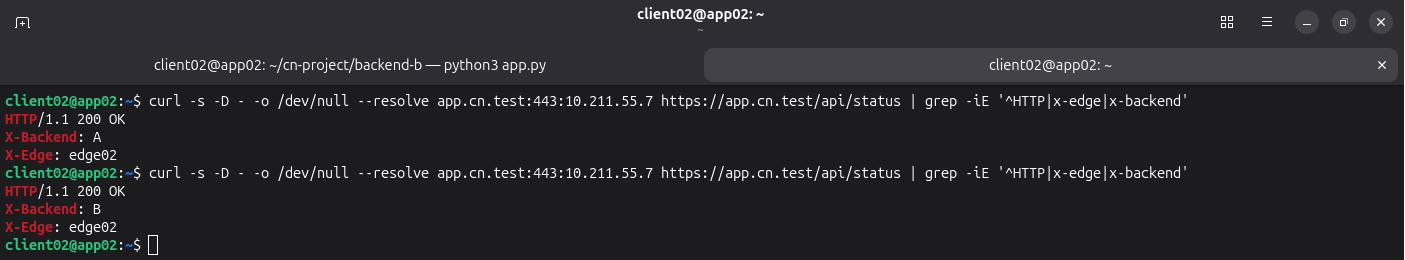
\includegraphics[width=\columnwidth]{p2_fig19_edge02_direct_test.png}
\caption{edge02 tested directly before the cutover.}
\label{fig:e-direct}
\end{figure}

\emph{Cutover.} Two clients ran a loop every 2\,s printing the IP curl connected to and the \cmd{X-Edge} header:
app02 as the \emph{cached} client and dns01 as the \emph{new-lookup} client, which flushed its cache right after the
record on both DNS servers was changed to \cmd{.7}. edge01's access log was followed at the same time.

\emph{Observed} (Fig.~\ref{fig:e-cut}). dns01 used edge01 until 03:16:19 and edge02 from the next request after its
flush at 03:16:21. app02 kept connecting to \cmd{10.211.55.6} (edge01) from its cache until 03:16:22 and switched to
\cmd{10.211.55.7} (edge02) at 03:16:24, when its cached answer expired. In edge01's log the last request from
\cmd{10.211.55.5} is at 03:16:19 and the last from \cmd{10.211.55.8} at 03:16:22; after that edge01 received nothing
and was \emph{drained}. edge02's access log contains 38 requests (8 from dns01 and 30 from app02). No request failed
during the migration. The cached client's lag depends on where in its 30\,s cache period the change falls; here its
cache expired about 3\,s after the flushed client moved, and in the worst case it would have been the full TTL.

\begin{figure*}[!t]
\centering
\subfloat[app02, cached client: edge01 until 03:16:22, edge02 from 03:16:24]{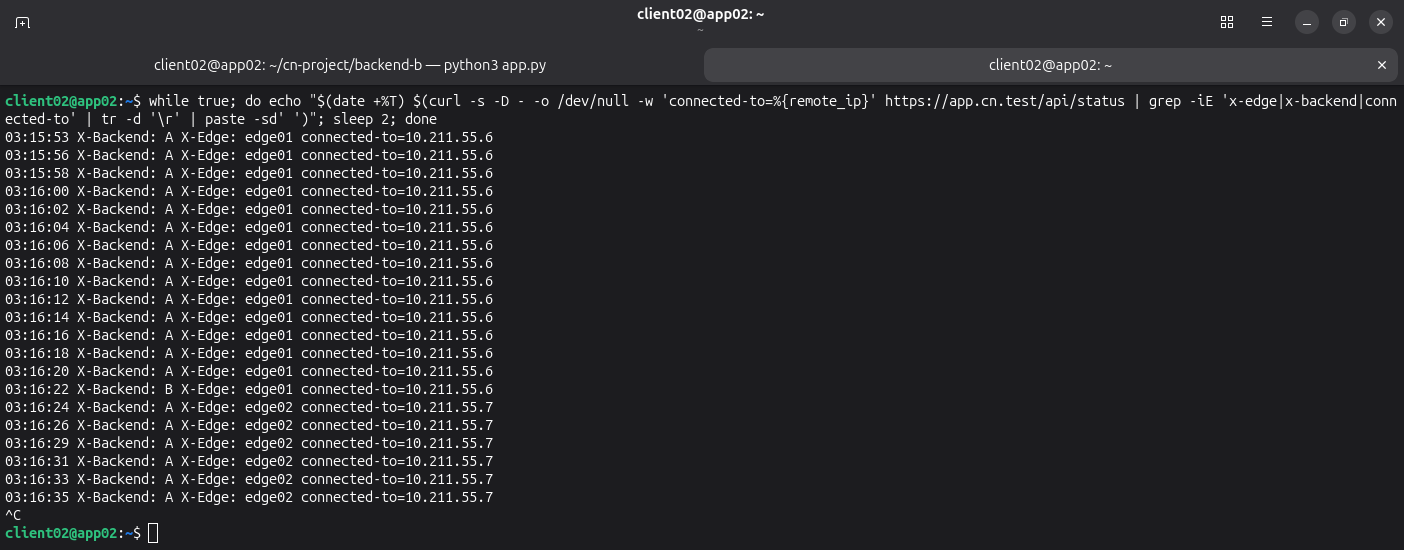
\includegraphics[width=0.49\textwidth]{p2_fig20_cutover_cached_client.png}}\hfill
\subfloat[dns01, flushed client: edge02 from the first request after the flush]{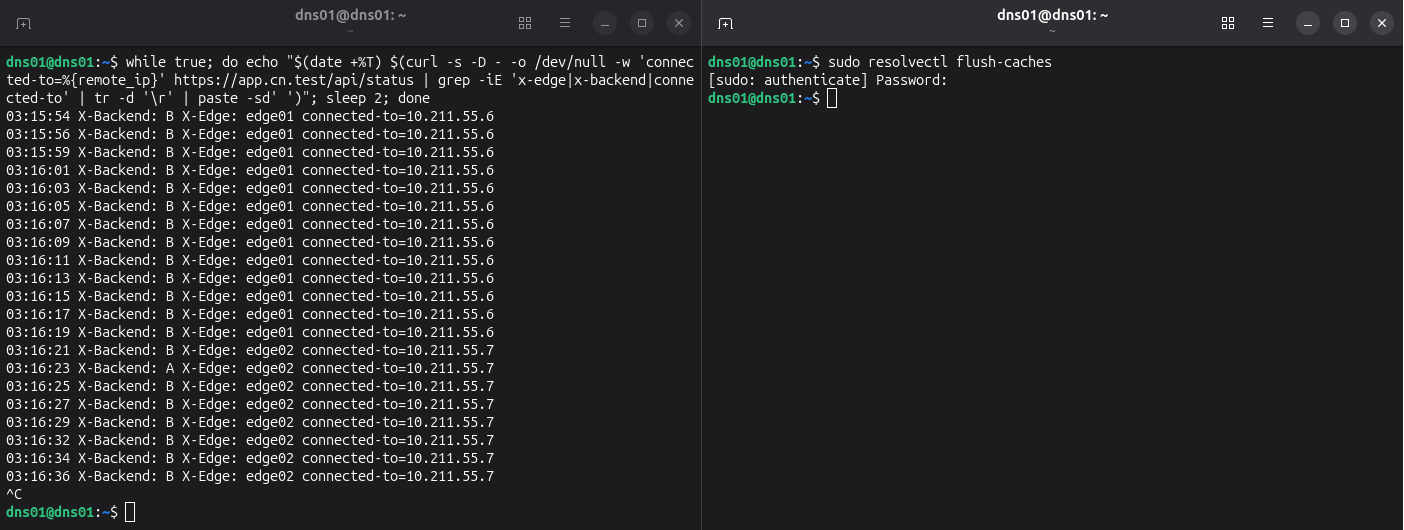
\includegraphics[width=0.49\textwidth]{p2_fig21_cutover_flushed_client.png}}\\
\subfloat[edge01 access log: requests from .5 and .8 stop, the old edge drains]{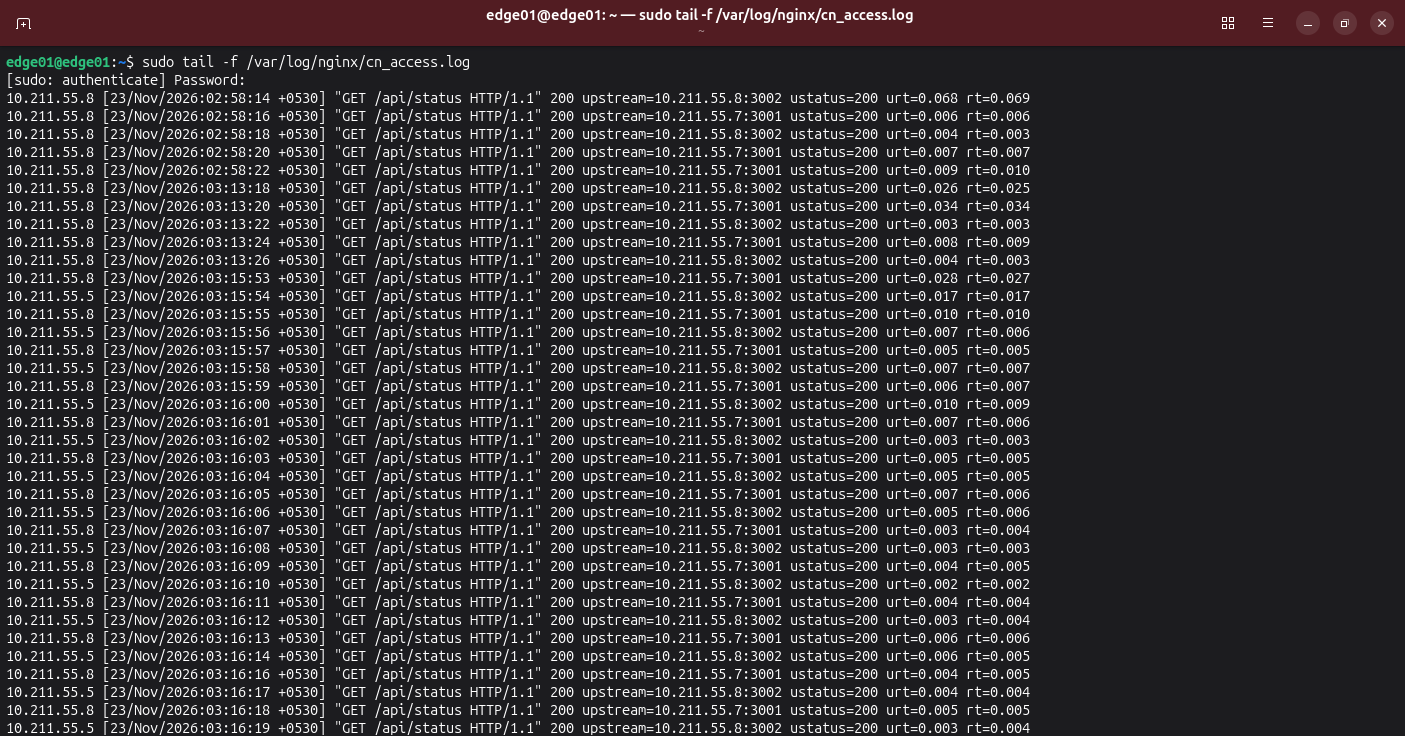
\includegraphics[width=0.62\textwidth]{p2_fig22_edge01_drained.png}}
\caption{Extension~E DNS-based cutover from edge01 to edge02.}
\label{fig:e-cut}
\end{figure*}

\emph{Rollback.} The record was set back to \cmd{.6} on both servers, the client cache flushed (\cmd{X-Edge: edge01}
again), and nginx on app01 stopped so that edge02 returns to standby.

% ---------------------------------------------------------------------
\subsection{Results Matrix}
Table~\ref{tab:matrix} summarises every required behaviour.

\begin{table}[!t]
\caption{Phase~2 Pass/Fail Matrix}
\label{tab:matrix}
\centering\footnotesize
\begin{tabularx}{\columnwidth}{@{}c Y l c@{}}
\toprule
Ext. & Requirement & Evidence & Result\\
\midrule
A & Backup resolver with identical records & Fig.~\ref{fig:a-direct} & \pass\\
A & Clients list both resolvers & \cmd{resolvectl} & \pass\\
A & Names resolve with primary stopped & Fig.~\ref{fig:a-failover}, pcap & \pass\\
A & DNS vs.\ application failure explained & Figs.~\ref{fig:a-dnsfail}, \ref{fig:a-appfail} & \pass\\
B & Short visible TTL (30\,s) & Fig.~\ref{fig:b-ttl} & \pass\\
B & Cached answer kept until TTL expiry & Fig.~\ref{fig:b-change} & \pass\\
B & Manual flush applies change at once & Fig.~\ref{fig:b-flush} & \pass\\
C & Only the edge reaches 3001/3002 & Figs.~\ref{fig:c-rules}, \ref{fig:c-after} & \pass\\
C & Rollback copy kept and restored & Fig.~\ref{fig:c-rollback} & \pass\\
D & Traffic routed only to healthy backend & Figs.~\ref{fig:d-down}, \ref{fig:d-log} & \pass\\
D & Balancing resumes after recovery & Fig.~\ref{fig:d-rec} & \pass\\
D & Remaining SPOF identified & Sec.~\ref{sec:limits} & \pass\\
E & Standby edge with same config & Fig.~\ref{fig:e-direct} & \pass\\
E & Cached clients lag, new lookups move & Fig.~\ref{fig:e-cut} & \pass\\
F & Systematic diagnosis method prepared & Sec.~\ref{sec:trouble} & Ready\\
\bottomrule
\end{tabularx}
\end{table}

% =====================================================================
\section{Troubleshooting Findings (Extension F)}\label{sec:trouble}
The faculty-injected fault is diagnosed bottom-up, one layer at a time and out loud, changing one thing at a time
(Table~\ref{tab:method}). Each layer has a distinct failure signature: \cmd{connection refused} means the host is up but
nothing listens; a \cmd{timeout} means a firewall DROP or a dead host; a curl error \cmd{(6)} points to DNS, \cmd{(60)} to
certificate trust, and an HTTP \cmd{502} proves that everything up to the edge works.

\begin{table}[!t]
\caption{Layer-by-Layer Diagnosis Method}
\label{tab:method}
\centering\footnotesize
\begin{tabularx}{\columnwidth}{@{}>{\raggedright\arraybackslash}p{1.1cm} Y >{\raggedright\arraybackslash}p{1.9cm}@{}}
\toprule
Layer & Command (from app02) & Healthy result\\
\midrule
DNS & \cmd{dig @.5 / @.7 app.cn.test} & NOERROR, 10.211.55.6\\
IP & \cmd{ping -c3 10.211.55.6} & replies\\
TCP & \cmd{nc -vz -w3 10.211.55.6 443} & succeeded\\
TLS & \cmd{openssl s\_client} \cmd{-verify\_hostname} & Verify return code 0\\
HTTP & \cmd{curl -D - .../api/status} & 200, A/B alternate\\
Behind edge & \cmd{nc} to :3001 and :3002; \cmd{cn\_error.log} & both succeed, no errors\\
\bottomrule
\end{tabularx}
\end{table}

Three drills, each a fault that actually occurred during Phase~2, are written up in
\cmd{evidence/troubleshooting/}:

\begin{itemize}
\item \emph{Drill 1: DNS service down.} Symptom: \cmd{Could not resolve host}. \cmd{dig} to the primary is refused,
yet ping to the edge works, so the layer is DNS (service). Fix: start dnsmasq on both servers.
\item \emph{Drill 2: one backend down.} Symptom: no error, but \cmd{X-Backend} is always B and one
\cmd{X-Upstream} lists two servers. The edge error log shows \cmd{connect() failed (111)} for \cmd{.7:3001}.
Layer: behind the edge. Fix: restart Backend~A. This fault is invisible without the Phase~2 headers and log format.
\item \emph{Drill 3: both backends down.} Symptom: \cmd{502 Bad Gateway} from nginx. DNS, TCP and TLS work, so the
layer is the application behind the edge. Fix: start both backends.
\end{itemize}

The other practised faults include a wrong DNS record, a wrong client resolver, nginx stopped, a DROP on port 443,
a wrong listen port, a mismatched certificate file, the CA removed from the trust store, the \cmd{api.cn.test} SAN
mismatch, a wrong upstream port, a backend bound to 127.0.0.1, a wrong firewall allow-list and a wrong system clock.

% =====================================================================
\section{Learning Summary}\label{sec:learning}

\emph{Extension A (backup DNS).} A resolver list gives redundancy only if every server holds identical records, and
the client resolver handles the failover itself: a stopped dnsmasq answers with ICMP port unreachable and
systemd-resolved moves to the next server and stays there. The key distinction is that a DNS failure stops the
request before any TCP connection exists, while an application failure lets DNS, TCP and TLS succeed and surfaces as
an HTTP 502 from the edge, so the first two commands of any diagnosis already separate the two.

\emph{Extension B (TTL).} The TTL is enforced by the client's caching resolver, not by the server. After a record
change, clients keep the old answer for up to one TTL, which the countdown made directly visible. A low TTL gives fast
changes at the cost of more queries; a high TTL does the opposite. Production migrations therefore lower the TTL at
least one old-TTL period before a change, switch the record, keep the old target alive for several TTLs, and raise the
TTL again afterwards~\cite{rfc1035,rfc2181}.

\emph{Extension C (isolation).} A host firewall turns ``the client should go through the edge'' from a convention into
an enforced rule, like a cloud security group that admits a port only from the load balancer. Rule order matters
because the first match wins, DROP looks like a dead host while REJECT fails fast, and a rollback copy taken before
the change makes the experiment safe to undo exactly.

\emph{Extension D (HA failover).} Open-source nginx learns that a backend is down only from failed real requests
(passive health checks). A refused connection is detected instantly, but a silent host is detected only by timeout, so
lowering \cmd{proxy\_connect\_timeout} from 60\,s to 2\,s is what makes failover fast. Retrying an idempotent request
on the next upstream hides the failure from the client, and headers such as \cmd{X-Upstream} are needed to see it at all.

\emph{Extension E (edge migration).} DNS-based cutover moves traffic with no client changes and no downtime, but
gradually: each client moves when its own cache expires, so the old edge must keep serving until its access log shows
no more traffic. The cutover also exposed hidden dependencies: the standby needed the same certificate and its own
firewall allow-list entry on the backends.

\emph{Extension F (troubleshooting).} A fixed bottom-up order turns an unknown fault into a sequence of yes/no
questions, and each tool's error message (refused, timed out, verify code, 502) maps to one layer. Instrumentation
added for the other extensions, namely query logging, upstream logs and the \cmd{X-*} headers, made several faults
diagnosable that would otherwise only look like ``it works, but differently''.

% =====================================================================
\section{Remaining Limitations}\label{sec:limits}
\begin{itemize}
\item The edge (edge01) remains a single point of failure; edge02 is a manually activated standby, not an automatic one.
\item app01 carries three roles (Backend~A, dns02, edge02), so losing that one VM removes several redundancies at once.
\item Health checks are passive only; active probing would need nginx Plus, HAProxy or a cloud load balancer.
\item The two DNS servers are synchronised by hand rather than through zone transfers or configuration management.
\item Edge failover through DNS is bounded by the TTL (30\,s) and by clients that ignore TTLs.
\item The certificate's SAN covers only \cmd{app.cn.test}, so HTTPS to \cmd{api.cn.test} fails hostname validation.
\item iptables rules are not persistent across reboots.
\end{itemize}

% =====================================================================
\section{Conclusion}
Phase~2 hardened the Phase~1 platform without rebuilding it. Name resolution survives the loss of the primary DNS
server, record changes behave predictably under a 30\,s TTL, backends accept traffic only from the edges, nginx removes
a failed backend within one request and restores it automatically, and traffic can be migrated to a standby edge with
DNS alone and without failed requests. All mandatory behaviours of Extensions A--E passed, the troubleshooting method
for Extension~F is prepared and rehearsed, and the edge remains the clearly identified next single point of failure
to eliminate.

% =====================================================================
\appendices
\section{Evidence Index}
\begin{table}[!h]
\centering\footnotesize
\begin{tabularx}{\columnwidth}{@{}l Y@{}}
\toprule
Folder & Contents\\
\midrule
\cmd{images/} & \cmd{p2\_fig01}--\cmd{p2\_fig23} screenshots (cropped copies for this report in \cmd{artifacts/figures/})\\
\cmd{wireshark/} & \cmd{phase2\_dns\_failover.pcapng}; also \cmd{phase2\_ha\_failover}, \cmd{phase2\_isolation\_blocked}, \cmd{phase2\_edge\_cutover} (.pcapng)\\
\cmd{vm\_logs/dns01/} & Phase~2 dnsmasq config, dnsmasq journal (Phase~1 config in \cmd{phase-1/evidence/vm\_logs/})\\
\cmd{vm\_logs/edge01/} & Phase~2 nginx config, \cmd{cn\_access.log}, \cmd{cn\_error.log} (Phase~1 config in \cmd{phase-1/})\\
\cmd{vm\_logs/app01/} & dns02 config and journal, edge02 config and logs, iptables before, applied (\cmd{iptables-ext-c-applied.rules}) and after\\
\cmd{vm\_logs/app02/} & iptables before, applied and after, \cmd{resolvectl} status\\
\cmd{troubleshooting/} & method and three drill write-ups\\
\cmd{architecture/} & Phase~2 topology and request-flow diagrams, architecture document\\
\bottomrule
\end{tabularx}
\end{table}

% =====================================================================
\begin{thebibliography}{9}
\bibitem{projdoc} ``Computer Networks Project: Private Network Service Platform,'' course project document, Newton School of Technology, Rishihood University, 2026.
\bibitem{rfc1035} P.~Mockapetris, ``Domain names -- implementation and specification,'' RFC~1035, IETF, Nov. 1987.
\bibitem{rfc2181} R.~Elz and R.~Bush, ``Clarifications to the DNS specification,'' RFC~2181, IETF, Jul. 1997.
\bibitem{rfc9293} W.~Eddy, Ed., ``Transmission Control Protocol (TCP),'' RFC~9293, IETF, Aug. 2022.
\bibitem{rfc8446} E.~Rescorla, ``The Transport Layer Security (TLS) protocol version 1.3,'' RFC~8446, IETF, Aug. 2018.
\bibitem{rfc9110} R.~Fielding, M.~Nottingham, and J.~Reschke, Eds., ``HTTP semantics,'' RFC~9110, IETF, Jun. 2022.
\bibitem{dnsmasq} S.~Kelley, ``dnsmasq(8) -- a lightweight DHCP and caching DNS server,'' manual page. [Online]. Available: \url{https://thekelleys.org.uk/dnsmasq/docs/dnsmasq-man.html}
\bibitem{nginxup} ``Module ngx\_http\_upstream\_module'' and ``Module ngx\_http\_proxy\_module,'' nginx documentation. [Online]. Available: \url{https://nginx.org/en/docs/}
\bibitem{iptables} ``iptables(8) -- administration tool for IPv4 packet filtering and NAT,'' Linux manual page.
\end{thebibliography}

\end{document}
